\documentclass[12pt]{thapathaliece}

% =========================================
%               Custom Variables
% =========================================
\newcommand\cUniversity{Tribhuvan University}
\newcommand\cDepartment{Institute of Engineering}
\newcommand\cCampus{Thapathali Campus}
\newcommand\cDocumentType{A MINOR PROJECT REPORT}  % Options: MAJOR/MINOR PROJECT PROGRESS/PROPOSAL REPORT
\newcommand\cTitle{Brain-Computer Interface for Text Entry using 
EEG Frequency Band Analysis}
\newcommand\cTitleShort{IEEE report Template and Guidelines}

% =========================================
%          Author Information
% =========================================
% Define only the authors you have (3 or 4)
% Leave \cSubmittedIV and \cSubmittedIVRoll empty for 3 authors

\renewcommand\cSubmittedI{Anup Ghimire}
\renewcommand\cSubmittedII{Rohit Dhourali}
\renewcommand\cSubmittedIII{Sudin Barakoti}
\renewcommand\cSubmittedIV{Swastik Rai}  % Leave empty for 3 authors, or add 4th author name

\renewcommand\cSubmittedIRoll{(38754)}
\renewcommand\cSubmittedIIRoll{(38777)}
\renewcommand\cSubmittedIIIRoll{(38785)}
\renewcommand\cSubmittedIVRoll{(38788)}  % Leave empty for 3 authors, or add 4th roll number

% =========================================
%          Faculty Information
% =========================================

\newcommand\cSupervisor{Er. Praches Acharya}
\newcommand\cSupervisorTitle{Project Supervisor}
\newcommand\cSupervisorDept{Department of Electronics and Computer Engineering}
\newcommand\cSupervisorAddress{Thapathali Campus, IOE}

%Project Coordinator Info
\newcommand\cProjectCoordinator{Er. Praches Acharya}
\newcommand\cProjectCoordinatorTitle{Project Coordinator}
\newcommand\cProjectCoordinatorDept{Department of Electronics and Computer Engineering}
\newcommand\cProjectCoordinatorAddress{Thapathali Campus, IOE}

%HOD Info
\newcommand\cHOD{Er. Umesh Kanta Ghimire}
\newcommand\cHODTitle{Head of Department}
\newcommand\cHODDept{Department of Electronics and Computer Engineering}
\newcommand\cHODAddress{Thapathali Campus, IOE}

%External Examiner Info
\newcommand\cExternalExaminer{Dr. Ram Kaji Budhathoki}
\newcommand\cExternalExaminerTitle{External Examiner}
\newcommand\cExternalExaminerDept{Professor,
	Department of Electrical and Electronics
	Engineering}
\newcommand\cExternalExaminerAddress{School of Engineering,
	Kathmandu University, Dhulikhel, Kavre}


% Date Formats
\newcommand\cDate{May 2026}
%\newcommand\cDateFull{March 6, 2026}



% Optional helper packages used by some guideline chapters
\usepackage{tcolorbox}
\usepackage{tikz}
\usepackage[english]{babel}
\usepackage[acronym]{glossaries}
\makeglossaries  
\usetikzlibrary{shapes.geometric, arrows.meta, positioning, shapes, fit, calc}
\usepackage{float}
\usepackage{algorithm}
\usepackage{algpseudocode}  
\usepackage{booktabs}

\usepackage{listings}
\usepackage{xcolor}

\definecolor{codegray}{rgb}{0.4,0.4,0.4}
\definecolor{codeblue}{rgb}{0.0,0.0,0.5}
\definecolor{codegreen}{rgb}{0,0.5,0}





% Glossary entries (define once, print later)

%% ABBREVIATIONS/ACRONYMS DEFINITIONS
% Use \gls{key} in text for first use (expands to full form + acronym)
% Subsequent uses show only acronym
% Use \Gls{key} for capitalized version
% Use \glspl{key} for plural
% Use \acrfull{key} to force full form + acronym
% Use \acrshort{key} to force acronym only

% ABBREVIATIONS/ACRONYMS DEFINITIONS
\newacronym{adc}{ADC}{Analog to Digital Converter}
\newacronym{bci}{BCI}{Brain Computer Interface}
\newacronym{bold}{BOLD}{Blood Oxygen Level Dependent}
\newacronym{ecog}{ECoG}{Electrocorticography}
\newacronym{eeg}{EEG}{Electroencephalogram}
\newacronym{erp}{ERP}{Event Related Potential}
\newacronym{fft}{FFT}{Fast Fourier Transform}
\newacronym{fmri}{fMRI}{Functional Magnetic Resonance Imaging}
\newacronym{hz}{Hz}{Hertz}
\newacronym{meg}{MEG}{Magnetoencephalography}
\newacronym{nirs}{NIRS}{Near Infrared Spectroscopy}
\newacronym{sar}{SAR}{Successive Approximation Register}
\newacronym{scp}{SCP}{Slow Cortical Potential}
\newacronym{smr}{SMR}{Sensorimotor Rhythm}
\newacronym{ssvep}{SSVEP}{Steady State Visual Evoked Potential}
\newacronym{vep}{VEP}{Visual Evoked Potential}


\newpage
\section*{\centering LIST OF ABBREVIATIONS}

\begin{tabular}{p{3cm} p{10cm}}
	AC	  & Alternating Current \\
	ADC   & Analog to Digital Converter \\
	BCI   & Brain Computer Interface \\
	BOLD  & Blood Oxygen Level Dependent \\
	DC	  & Direct Current \\
	ECoG  & Electrocorticography \\
	EEG   & Electroencephalogram \\
	ERP   & Event Related Potential \\
	FFT   & Fast Fourier Transform \\
	fMRI  & Functional Magnetic Resonance Imaging \\
	Hz    & Hertz \\
	MEG   & Magnetoencephalography \\
	NIRS  & Near Infrared Spectroscopy \\
	SAR   & Successive Approximation Register \\
	SCP   & Slow Cortical Potential \\
	SMR   & Sensorimotor Rhythm \\
	SSVEP & Steady State Visual Evoked Potential \\
	UART  & Universal Asynchronous Receiver/Transmitter\\
	VEP   & Visual Evoked Potential \\
\end{tabular}


%\input{src/frontmatter/symbols}



\begin{document}
% =====================
% FRONTMATTER
% =====================

\input{src/frontmatter/_coverBase}
\input{src/frontmatter/_coverWithSupervisors}

\clearpage
\pagenumbering{roman}

\input{src/frontmatter/certificate}
\input{src/frontmatter/declar}
\input{src/frontmatter/copyright}



% Standard frontmatter
% Copyright Page
\chapter*{ACKNOWLEDGEMENT}
\phantomsection
\addcontentsline{toc}{chapter}{ACKNOWLEDGEMENT}

We would like to express our sincere gratitude to the Department of Electronics and Computer Engineering, Institute of Engineering, Thapathali Campus, for providing us the opportunity to carry out this minor project. This project has helped us gain practical knowledge and improve our understanding of theoretical concepts.

We would like to thank our project supervisor \textbf{Er.Praches Acharya} for his valuable guidance, continuous support, and helpful suggestions throughout the project period. His guidance helped us to stay on the right path and successfully complete this work.

We are also thankful to all the teachers and staff members of the department for their support and cooperation during the project. Their encouragement and assistance played an important role in completing this project.
We would like extend our sincere thanks to our friends and family members for their motivation, cooperation, and moral support throughout the project duration.

\vspace{1em}
\noindent \authorTable


\chapter*{ABSTRACT}
\phantomsection
\addcontentsline{toc}{chapter}{ABSTRACT}


\bigskip

A Brain-Computer Interface (BCI) lets a person control a computer or device directly using brain signals which are recorded from the scalp using EEG electrodes. In this project, a low cost EEG based BCI typing system is designed using eye blinks and beta brain waves as control signals unlike complex systems that uses visual stimuli or machine learning, this system focuses on simplicity, affordability and ease of use. EEG signals are collected using electrodes and processed with basic signal processing techniques. Eye blinks create large changes in the EEG signal and are used for traversing the key in on-screen typing interface and focus state of brain can select the key. Waves generated from the brain sensed by electrodes are passed through analog filter and amplifiers to acquire adequate signal for computation of Fast Fourier Transform (FFT) on arduino microcontroller, where the obtained frequency information is used to differentiate the eye blink and focus state of brain which is the basis of using on-screen typing interface for our BCI system. A simple stimulus based method is able map these signals to typing and selection of commands  for interfacing. BCI can be helpful for people with movement difficulties and for situations where hands free control is preferred.


\vspace{1em}
\noindent\textit{\textbf{Keywords}: BCI, Electroencephalogram (EEG), Fast Fourier Transform (FFT), Signal Processing, Typing Interface}

\input{src/frontmatter/toc}
% ABBREVIATIONS/ACRONYMS DEFINITIONS
% Use \gls{key} in text for first use (expands to full form + acronym)
% Subsequent uses show only acronym
% Use \Gls{key} for capitalized version
% Use \glspl{key} for plural
% Use \acrfull{key} to force full form + acronym
% Use \acrshort{key} to force acronym only

% ABBREVIATIONS/ACRONYMS DEFINITIONS
\newacronym{adc}{ADC}{Analog to Digital Converter}
\newacronym{bci}{BCI}{Brain Computer Interface}
\newacronym{bold}{BOLD}{Blood Oxygen Level Dependent}
\newacronym{ecog}{ECoG}{Electrocorticography}
\newacronym{eeg}{EEG}{Electroencephalogram}
\newacronym{erp}{ERP}{Event Related Potential}
\newacronym{fft}{FFT}{Fast Fourier Transform}
\newacronym{fmri}{fMRI}{Functional Magnetic Resonance Imaging}
\newacronym{hz}{Hz}{Hertz}
\newacronym{meg}{MEG}{Magnetoencephalography}
\newacronym{nirs}{NIRS}{Near Infrared Spectroscopy}
\newacronym{sar}{SAR}{Successive Approximation Register}
\newacronym{scp}{SCP}{Slow Cortical Potential}
\newacronym{smr}{SMR}{Sensorimotor Rhythm}
\newacronym{ssvep}{SSVEP}{Steady State Visual Evoked Potential}
\newacronym{vep}{VEP}{Visual Evoked Potential}


\newpage
\section*{\centering LIST OF ABBREVIATIONS}

\begin{tabular}{p{3cm} p{10cm}}
	AC	  & Alternating Current \\
	ADC   & Analog to Digital Converter \\
	BCI   & Brain Computer Interface \\
	BOLD  & Blood Oxygen Level Dependent \\
	DC	  & Direct Current \\
	ECoG  & Electrocorticography \\
	EEG   & Electroencephalogram \\
	ERP   & Event Related Potential \\
	FFT   & Fast Fourier Transform \\
	fMRI  & Functional Magnetic Resonance Imaging \\
	Hz    & Hertz \\
	MEG   & Magnetoencephalography \\
	NIRS  & Near Infrared Spectroscopy \\
	SAR   & Successive Approximation Register \\
	SCP   & Slow Cortical Potential \\
	SMR   & Sensorimotor Rhythm \\
	SSVEP & Steady State Visual Evoked Potential \\
	UART  & Universal Asynchronous Receiver/Transmitter\\
	VEP   & Visual Evoked Potential \\
\end{tabular}


%\glsaddall

% Start a new page
\cleardoublepage

% Add a title without making a chapter
\section*{LIST OF ABBREVIATIONS} % keeps it small like a section
\addcontentsline{toc}{section}{LIST OF ABBREVIATIONS} % appears in TOC

\glsaddall
% Print the glossary entries
\printglossary[type=\acronymtype,style=long, title={}]
\clearpage

% =====================
% MAINMATTER
% =====================
\clearpage
\pagenumbering{arabic}

\chapter{Introduction}

%\noindent\textbf{CHAPTER GUIDE:} Purpose: set context, define the problem, and state objectives + scope. Must include: Background, Problem statement, Objectives, Scope and limitations. How to write: mention domain + current approaches; quantify gaps with metrics. LaTeX: Cite with cite key, reference figures and tables. General rules: formal/technical style; cite non-trivial claims; reference figures/tables in text.

\section{Background}

% Test abbreviations and symbols
%This project uses \gls{ga} and \gls{ml} techniques \cite{deb2002nsga}. We also implement \gls{rl} with \gls{api} integration. The \gls{cpu} and \gls{gpu} work together for processing.

%Research shows optimization methods are crucial in modern computing \cite{smith2020}. Following IEEE guidelines \cite{ieee2022author, ieee2021editorial}, we implement state-of-the-art algorithms.

%The learning rate \gls{symb:alpha} is crucial, and we use discount factor \gls{symb:gamma}. Standard deviation \gls{symb:sigma} helps measure variance with mean \gls{symb:mu}.

Brain-Computer Interface (BCI) is a technology that allows a human to directly control a computer or other external device through activity in the brain. The idea of BCI has gained interest, not only because of its novelty, but also because of its practical significance to individuals who may be unable to interact with devices such as keyboards, mice, or touchscreens. So BCI has gained significance as a research area for its application in assistive communication, rehabilitation, and hands free computer interaction.

Electroencephalography (EEG) is commonly used for non invasive BCI systems as it records the electrical activity of the brain using electrodes placed on the scalp. It is the go to method because it is safe, low cost and portable but EEG signals are very small and easily affected by noise, so careful signal processing is necessary. 

Different BCI methods focus on certain EEG features, such as event related signals, visual responses or natural brain rhythms, to interpret the user’s intent such as alpha brain waves, which appear in the 8-12 Hz range and are usually linked to relaxed or unfocused states. As the person becomes attentive, there will be an increase in the beta wave, thus making it possible to use it as a control signal to determine the level of concentration. Eye blinks create signals that are very clear in the EEG recording. They can be used as control signals. Through the combination of the beta wave and the eye blinks, we will be able to develop a reliable BCI control mechanism without having to rely on classification methods. This project is an extension of that concept.
This system applies simple signal processing techniques like filtering and frequency analysis while avoiding or using few expensive equipment and advanced complex methods.

\section{Motivation}
The motivation for this project comes from the need for affordable and easy to use assistive technologies that support hands free communication for people in need. Our knowledge on signal filtering, processing and many other important elements can be implemented which enhances our capability. Beyond technology and skill it also serves in building and advancing our society by empowering the individuals with tool to communicate, interact and participate normally in regular life.

Another motivation is to explore whether BCI control can be achieved using basic EEG signals and low cost hardware. When eye blinks big potential spike is formed making the easiest EEG features to detect and understand compared to other brain signals. Using these signals along with simple processing techniques like filtering and Fast Fourier Transform (FFT), it is possible to build a BCI system that is easy to set up and use.

In addition, the motive behind the development of this project was to gain practical experience in EEG signal acquisition and processing. Development of a prototype of the BCI typing interface provided us with an understanding of the practical problems faced such as noise, constraints in hardware, economics, etc. As a result, this project has produced a prototype of the BCI system using very basic techniques in machine learning and hardware.

\section{Problem Statement}
Typing through regular computing relies on the use of physical components such as keyboards and mouses; however, these physical components cannot be utilized by individuals suffering from motor disabilities and situations that require more physical movement than what the individual can manage. Although brain-computer interface (BCI) solutions may provide a viable solution to this problem, most EEG-based brain-computer interface typing systems require expensive components and sophisticated machine learning algorithms that rely on huge amounts of data, thus making it impossible to use in low-budget settings.

The main problem that our project aims to address is the absence of a simple and affordable BCI typing system that works with simple EEG hardware and fundamental signal processing techniques. On the other hand, the important element to explore is whether eye blink detection and beta wave analysis can reliably control a basic typing or text selection interface without advanced classification algorithms and the difficult challenge is to extract usable control signals from noisy EEG data with few use of electrode while maintaining the system's reliability and usability. This project aims to solve this problem by designing and testing a low complexity EEG based BCI typing system suitable for educational and assistive purposes.


\section{Objectives}
The main objectives of this project are as follows:
\begin{itemize}
	\item To design a simple and low cost EEG based Brain-Computer Interface system
	\item To analyze EEG frequency bands using basic filtering and FFT
	\item To develop a basic text entry using detected EEG signals.
\end{itemize}



\section{Scope and Limitations}
This project focuses on designing and building a simple EEG based BCI typing or text selection system using eye blink detection and beta wave analysis via non invasive EEG signal recording, digital filtering, FFT based feature extraction and basic stimuli based decision making. Only a one EEG channel is used to make the system simple and cheap.

The project is not meant to attain fast typing speeds or be accurate on the same standards used commercially. There will be no incorporation of advanced machine learning and extensive testing for clinical validation. The project will serve the main purpose of educational and experimental demonstration of BCI principles and concepts.

The applications of this BCI System are:\begin{itemize}
	\item Assistive communication for people with limited motor abilities
	\item Hands free computer control where keyboards or mice are not practical
	\item Educational demonstrations for learning EEG signal processing and BCI fundamentals
	\item Student and research projects focusing on low cost neuroscience or biomedical engineering experiments
	\item Experimental platforms for further development of more advanced BCI.
\end{itemize}

\chapter{LITERATURE REVIEW}

\section{Existing Works}
Brain-computer interfaces, are systems that let a person communicate with a computer using signals from the brain. These systems read brain activity and turn it into signals that a computer or device can understand, without needing things like a keyboard or mouse. BCIs can be grouped based on how they record brain signals. The main types include:\begin{itemize}
	\item \gls{eeg}
	\item Functional magnetic resonance imaging (fMRI)
	\item Near infrared spectroscopy (NIRS)
	\item Magnetoencephalography (MEG)
	\item Electrocorticography (ECoG)

\end{itemize}

EEG is a non-invasive method that records the electrical activity of the brain using electrodes placed outside the head in the scalp. ECoG is different because it is invasive and places electrodes directly on the surface of the brain to measure electrical activity. ECoG can give better accuracy than EEG, but because it is invasive, but this requires extensive surgery and includes risk to the user. MEG, fMRI, and NIRS are also non-invasive methods, but these require big industrial equipment. MEG measures the magnetic fields created by brain activity. fMRI uses strong electromagnetic fields and in BCI applications usually measures blood oxygen level dependent (BOLD) changes linked to neural activity. NIRS uses infrared light that can pass a short distance through the skull and measures the reflected light. More detailed descriptions of all these methods can be found in \cite{nicolas2012bci}.

\section{EEG Based BCI}
Focusing again on EEG based BCIs, there are several types of brain signals that can be used to send commands to a computer or other device. Some common examples include sensorimotor rhythms (SMRs), visually evoked potentials (VEPs), and slow cortical potentials (SCPs) . Each of these signals works in a different way and is useful for different kinds of BCI systems. In many practical and research based applications, VEPs and SMRs are among the most widely used because they can provide clear control signals and are well studied in the field. For this reason, these two EEG signal types are especially important and will be described in the following sections.

Visual evoked potentials, often called VEPs, are brain responses that appear when a person sees a visual stimulus. These signals can be observed from the occipital region, which is located at the back of the head and is strongly related to visual processing. When the visual stimulus flashes repeatedly at a constant frequency, the brain produces a repeating response of the identical frequency. This type of response is known as a steady state visually evoked potential, or SSVEP. In this type of system the user selects commands by looking a particular flickering pattern.

Even though VEP based systems have been extensively studied for BCI applications, this is not the emphasis of the current study. The current study emphasizes a different approach to VEP. An instance of SSVEP based application is an interface that resembles a keyboard where each character corresponds to a light source which flickers at a distinct frequency. It is possible to know what character the user is focused on by analyzing the frequency domain components of the EEG signal of the user. This allows us to determine the selected character based on the dominant frequency component of the occipital EEG signal  \cite{hwang2012ssvep}.


\section{Brain Waves and Their Relevance to the Proposed BCI System}
Electroencephalography (EEG) is an electrical activity of the brain registered in the form of waves, which belong to certain frequency ranges and represent particular mental or physiological conditions of a person. Delta waves (0.1 – 3 Hz) are the slowest waves that appear during deep dreamless sleep or when a person is unconscious. Theta waves (4 – 7 Hz) are associated with creative work, imagination, memory recollection and light sleeping or dreaming. They usually appear when a person's mind is relaxed and inwardly focused. Alpha waves (8 – 12 Hz) appear when a person is awake and relaxed. Such waves increase when a person's eyes are closed and decrease when he/she concentrates on something. Low beta waves (12 – 15 Hz) indicate relaxed but focused mental activities while mid range beta waves (16 – 20 Hz) reflect active thinking, problem solving and high awareness of the environment. High beta waves (21 – 30 Hz) appear when a person is highly alert, stressed or agitated. Gamma waves (30 – 100 Hz) are associated with higher mental processes like information processing, learning and memory integration. In the case of the suggested brain-computer interface (BCI) system, beta waves are to be used as control waves because they are clearly distinguished by their changes between relaxed and focused states allowing a simple and reliable interaction through the EEG-based interface. Although the other waves are not used for controlling the device directly, knowledge about all waves is crucial for proper filtering of noise and detecting beta waves activity.

\newpage
\begin{table}
	\centering
	\caption{\centering EEG frequency bands and associated mental states-Image Source: M.G.N.Garcia et al \cite{malmivuo1995bioelectromagnetism})}
	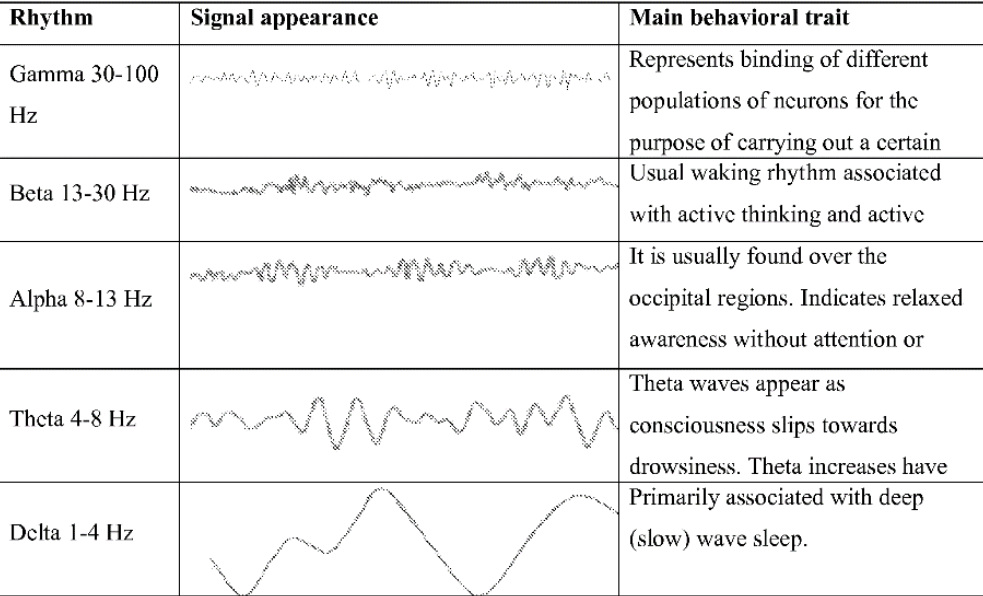
\includegraphics[width = 14cm]{src/images/figures/eeg_frequency_bands.png}
\end{table}

\vspace{10pt}
\section{Electroencephalography}
An EEG, or electroencephalogram, is a machine that can measure the tiny electrical signals our brain produces. We put small electrodes on the scalp to record these signals. People use EEG for many things like checking if someone is awake, seeing how they react to things around them, or finding sleep and brain problems. Lately, scientists started using EEG signals to control computers, which is called a BCI system \cite{vidal1973bci}.

The signals an EEG picks up depend on where the electrodes are placed and what the brain is doing at that moment. This is because different parts of the brain do different jobs. The most common way to put the electrodes on the head is called the 10-20 system \cite{malmivuo1995bioelectromagnetism}.

\begin{figure}
	\centering
	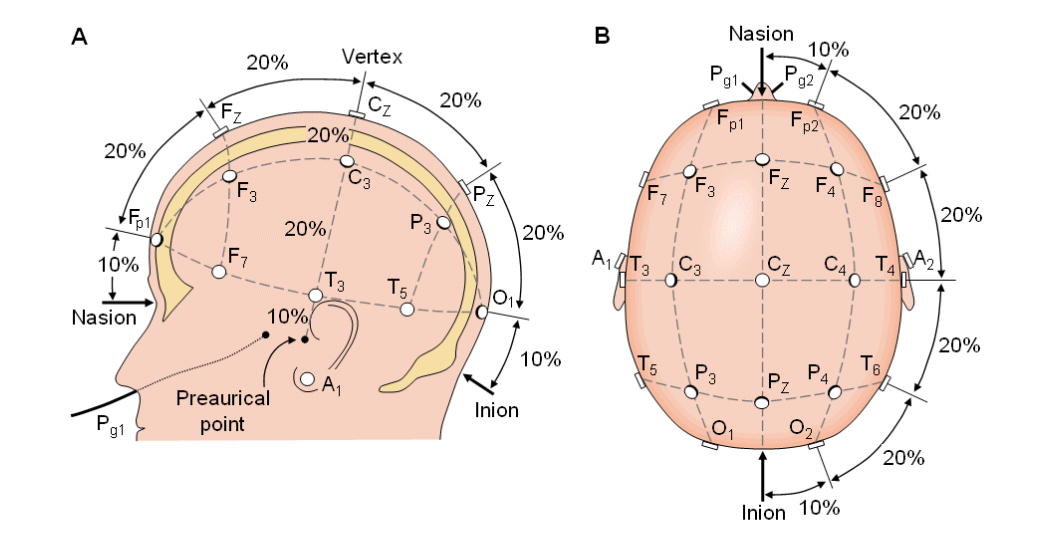
\includegraphics[width = 14cm]{src/images/figures/electrode_placement.png}
	\caption{\centering An example of the stimulation frequency arrangements (Image from H. Han Jeong \cite{hwang2012ssvep})}
\end{figure}

\chapter{REQUIREMENTS ANALYSIS}
\label{chap:requirements}

\section{Biopotential Electrodes}
Biopotential electrodes are used to measure small electrical signals produced inside the human body. These signals come from active cells such as brain cells and muscle cells. In EEG systems, two electrodes are used for each channel to measure the changing voltage on the scalp. This can be done by measuring the voltage between two points on the head, called bipolar configuration, or between one point on the head and a reference point like the ear, called unipolar configuration \cite{malmivuo1995bioelectromagnetism}.

Biopotential electrodes are mainly divided into two types: wet electrodes and dry electrodes. Wet EEG electrodes are usually small cup shaped electrodes filled with conductive gel. The gel helps the electrode make good contact with the scalp, even through hair. Dry electrodes do not use gel. Instead, they have small teeth like structures that pass through the hair and touch the scalp directly.

The problem with wet electrodes is that the gel can dry out affecting the signal quality and and it also causes skin irritaiton in some patients. Dry electrodes are generally more comfortable and easier to use because they do not require gel. However, they are more affected by body movement and usually have higher resistance between the skin and the electrode \cite{saab2011drywet}.

\begin{figure}[htbp]
	\centering
	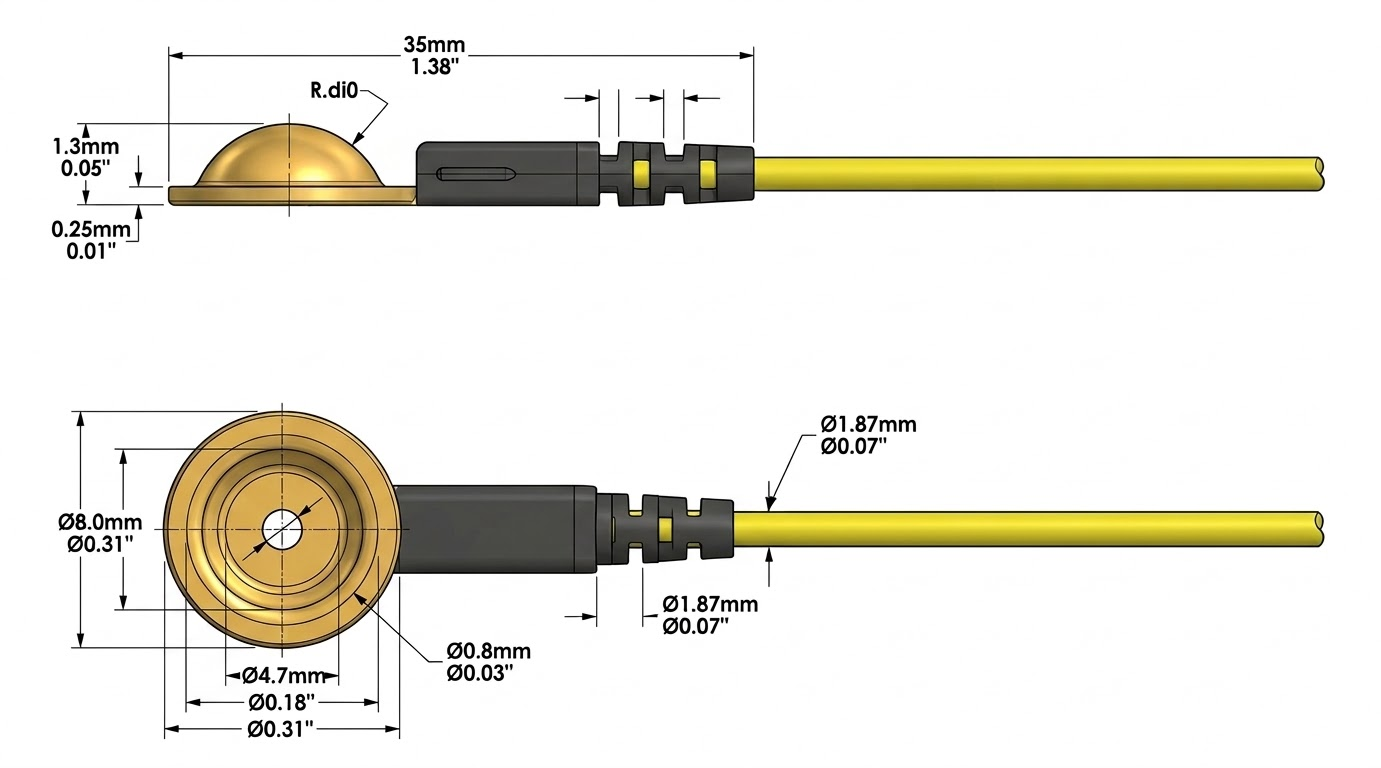
\includegraphics[width=0.45\textwidth]{src/images/figures/wet_cup_electrodes.png}
	\caption{\centering Wet EEG cup electrodes}
	\label{fig:wetElectrodes}
\end{figure}

EEG electrodes can also be made from different materials, such as silver/silver chloride, gold, silver, stainless steel, and tin. Reusable EEG electrodes are often expensive and can cost ten dollars or more per electrode \cite{biomedical2018electrodes}. To reduce the overall cost of the project, low cost and homemade electrodes were used.

Another way to classify EEG electrodes is as active or passive. Active electrodes include a small amplifier near the electrode itself. This helps reduce noise caused by poor contact with the skin and movement of wires \cite{gtec2018comparison}. Passive electrodes do not have this amplifier and are connected directly to the bio signal amplifier using long wires.


\section{Instrumentation Amplifier}
An instrumentation amplifier is used to amplify very small EEG signals obtained from the scalp electrodes. Brain signals are very weak and cannot be directly processed by filters or other circuits. Therefore, an instrumentation amplifier is used as the first stage of signal conditioning in this project.

In this system, the AD620 instrumentation amplifier is used because it is specially designed for low level bio potential signal amplification such as EEG. AD620 has high input impedance, which prevents loading of the electrodes and helps maintain signal quality. It also has high common mode rejection, which reduces common mode noise such as power line interference and motion artifacts.

\begin{figure}[H]
	\centering
	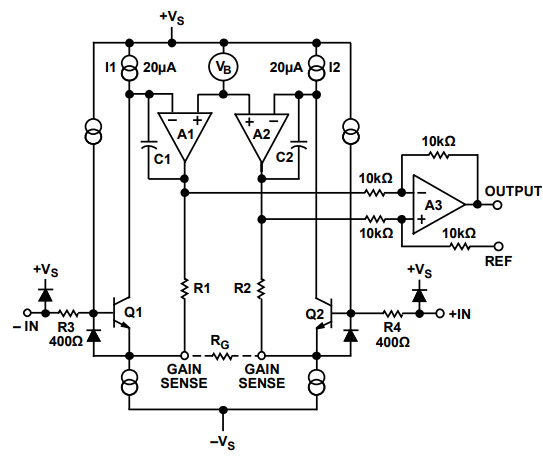
\includegraphics[width = 14cm]{src/images/figures/ad620_schematic.png}
	\caption{\centering Simplified Schematic of AD620 Source: \cite{ad620datasheet}}
\end{figure}

The gain of AD620 can be easily adjusted using a single external resistor, which makes the circuit simple and flexible. AD620 also operates with low noise, low power
consumption, and stable performance, making it suitable for continuous EEG signal acquisition.

By using the AD620 instrumentation amplifier, the small voltage difference between EEG electrodes is amplified accurately while rejecting common noise signals. This
improves signal clarity and makes the EEG signal suitable for further filtering and processing in the Brain-Computer Interface system.

\section{Types of Filters}
The role of filters in the EEG system is to remove noise and only allow the desired signals to be detected. The signals in the EEG are quite weak and susceptible to any noise. Some of the noises that can affect the EEG signals include power line interference and muscle movements among others. Therefore, the use of filters in signal conditioning is quite crucial.

Band pass filter is one of the filters used in the current project. In the case of band pass filter, only the required frequency of the EEG is allowed to pass through the filter. It eliminates slow drift and high frequency noises from the signal.

Low pass filter is used to eliminate high frequency noise. The high frequency noise includes muscle activity and external electrical interference.

High pass filter is employed in order to get rid of very low frequency noise. These kinds of noises include body movements and baseline drift.

In the current project, simple analog filters are used. They are simple to design and therefore suitable for low cost systems. They eliminate enough noise in order to detect eye blink and basic EEG frequencies.

\section{Arduino Microcontroller}
When the signal from the electrodes is converted into digital form, the microcontroller takes the samples and processes them within small time intervals. The initial signal processing functions such as amplitude thresholding are performed in the time domain. In order to perform frequency domain analysis, the microcontroller applies Fast Fourier Transform (FFT) algorithm on the digital EEG signal. As the result of the FFT analysis, the microcontroller detects eye blinks because eye blinks produce low frequencies.

In case of receiving valid brain or eye blink commands, the microcontroller uses predefined algorithms to make decisions and produces corresponding output signals. The outputs generated by the microcontroller can be used to control external devices like a cursor, virtual keyboard, or LED lights. Moreover, the microcontroller manages data communication between a computer or display device and the microcontroller. Therefore, the microcontroller is responsible for performing data acquisition, signal processing, decision making, and controlling devices within the BCI project.

\section{FFT and MATLAB (Signal Processing and Visualization)}
Fast Fourier Transform (FFT) is adopted in this work to transform the input EEG signal from time domain to frequency domain since frequency domain analysis is necessary to distinguish and extract certain frequency bands in the EEG signal, especially the beta band (12-30 Hz) that is related to relaxation and attention.

EEG signals obtained from Arduino are analyzed in MATLAB in which FFT is implemented to compute the power spectral density of the input signal. Depending on the strength of the beta band in the EEG signals, the mental state of the user can be determined.

MATLAB plotting tools can be used to plot the time domain signal as well as the frequency spectrum of the input EEG signals. This will facilitate performance analysis and validation of the implemented signal processing techniques.

\chapter{SYSTEM ARCHITECTURE AND METHODOLOGY}

\section{System Block Diagram/Architecture}
\vspace{20pt}
\begin{figure}[H]
	\centering
	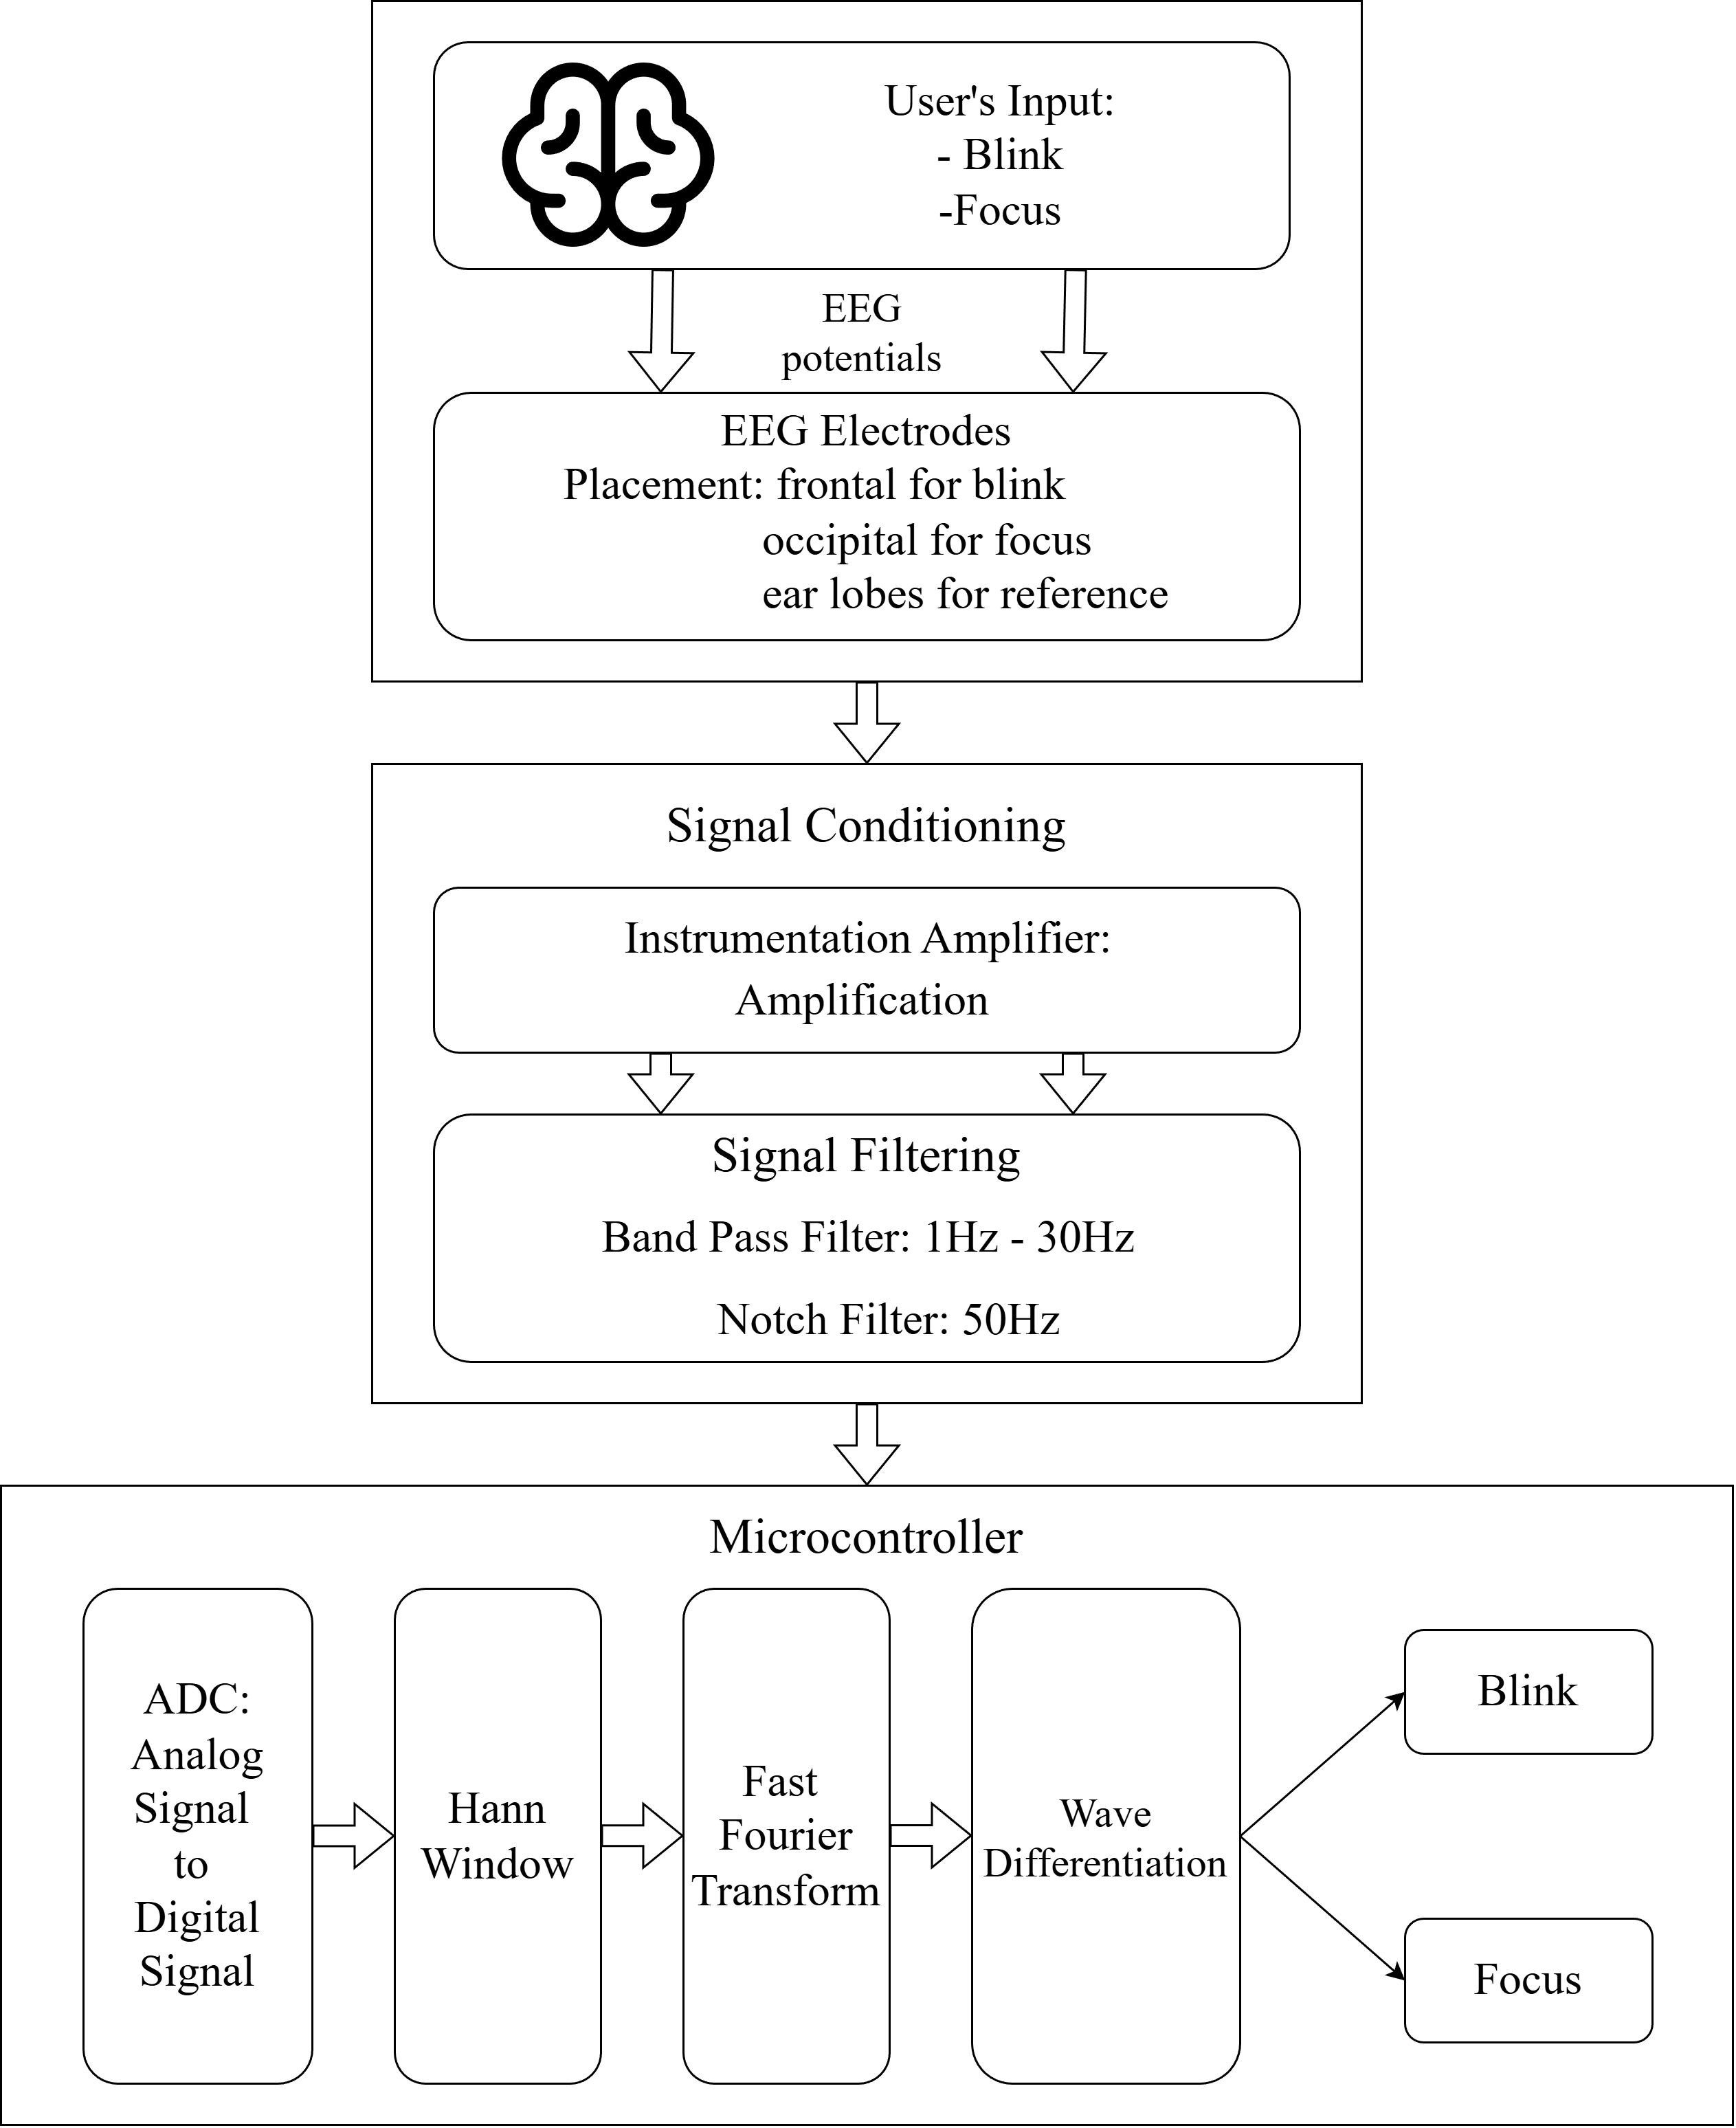
\includegraphics[width = 14.5cm, height=19.5cm]{src/images/figures/system_architecture.png}
\caption{System Block Diagram of the Brain-Computer Typing Interface}
\label{system_block_diagram}
\end{figure}

\newpage
\section{ Working Principle}
Brain Computer Interface (BCI) system is responsible for sensing, amplifying, filtering, and interpreting brain electrical signals for controlling external devices. EEG signals are sensed by electrodes attached to the scalp. The weak signals are amplified using Instrumentation Amplifier (AD620). Band pass filter such as Butterworth filter is used to filter out the required frequency signals and artifact as well as muscle activity.

Filtered signals are further converted into digital signals through ADC port of Arduino. Signal frequencies are analyzed using software algorithms that help in identifying visual stimuli that the user is concentrating on. This system is very sensitive, noise free and interference free.

More precisely, EEG electrodes are placed on the scalp at frontal and occipital regions to capture signals related to eye blinks and brain activity. A large voltage change appears in the EEG signal when the user performs an intentional eye blink. The proposed BCI typing system works by detecting eye blinks and changes in beta wave activity from EEG signals to control a typing or selection interface but beta wave activity varies depending on the user’s level of focus or relaxation and is mainly observed in the occipital region of the brain.

The EEG signals collected from the electrodes are first amplified and conditioned using an analog front end circuit then these signals are passed through analog filters including high pass and low pass to remove unwanted noise, baseline drift and power line interference. Then the clean EEG signals are converted into digital form using an analog to digital converter.

In the digital stage, the system stores the sampled EEG data in short time windows. Eye blinks are detected directly from the time domain signal using amplitude thresholding techniques and based on predefined thresholds, the system determines whether the user is focused or relaxed. For beta wave analysis, Fast Fourier Transform (FFT) is applied to the observed EEG data to calculate the power in the beta frequency band (12-30 Hz). If blink and beta states are detected then it is processed by a rule based decision logic, which translates them into typing or selection actions on the user interface.

\newpage
\section{Flowchart of Proposed System Architecture}
\vspace{18pt}
\begin{figure}[H]
	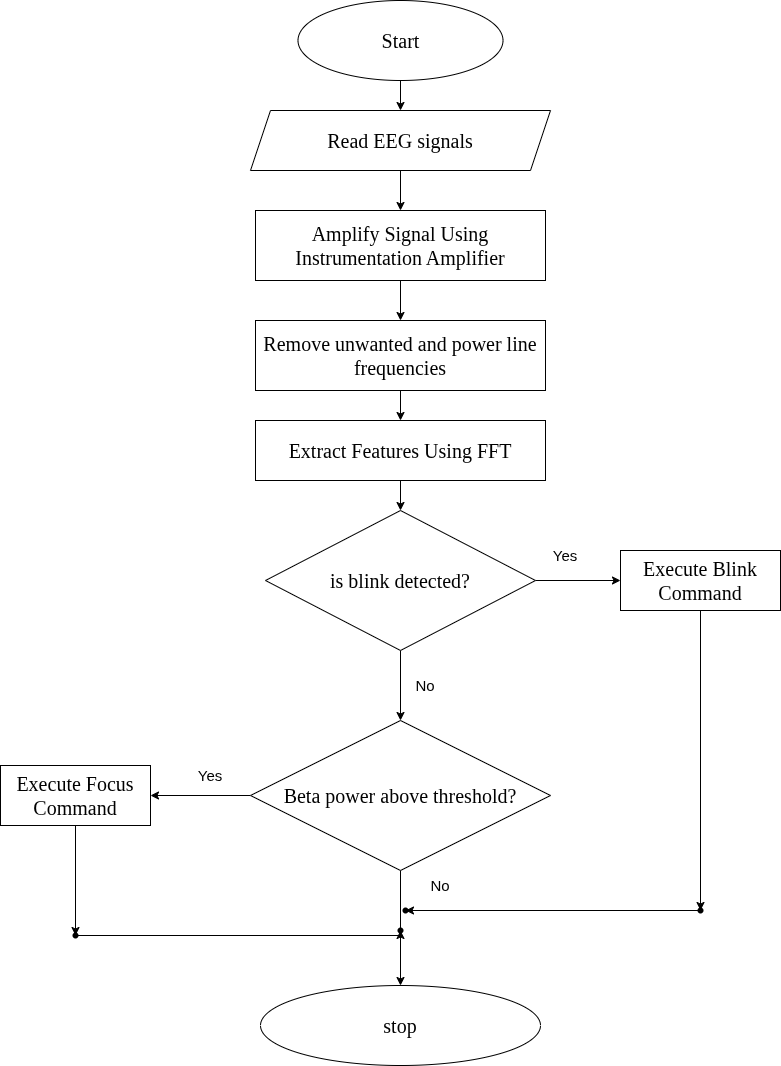
\includegraphics[width = 14cm, height = 21.5cm]{src/images/figures/flowchart.png}
	\vspace{10pt}
	\caption{Flowchart of Proposed System Architecture}
	\label{flowchart}
\end{figure}

\newpage
This flowchart illustrates the operation of the proposed EEG-based BCI system. The system acquires EEG signals, amplifies them using an instrumentation amplifier, and removes unwanted noise and power-line interference through filtering. FFT is then applied to extract relevant features. Based on these features, the system first checks for blink detection to execute a blink command; if no blink is detected, it evaluates beta-band power to determine focus and execute the corresponding focus command, after which the process ends.

\section{FFT flowchart for Arduino Program}
\tikzset{
	startstop/.style={
		ellipse,
		draw=black, thick,
		minimum width=5cm,
		minimum height=0.9cm,
		align=center,
		font=\small
	},
	process/.style={
		rectangle,
		draw=black, thick,
		minimum width=8cm,
		minimum height=1cm,
		align=center,
		font=\small,
		inner sep=6pt
	},
	decision/.style={
		diamond, aspect=3,
		draw=black, thick,
		minimum width=7cm,
		align=center,
		font=\small,
		inner sep=2pt
	},
	arrow/.style={-{Stealth[length=6pt]}, thick},
}
%% ════════════════════════════════════════════════════════
%%  PAGE 1 — Interrupt Service Routine
%% ════════════════════════════════════════════════════════
\begin{figure}[H]
	\centering
	\begin{tikzpicture}[node distance=0.65cm]
		
		\node (isrstart) [startstop]                        {Timer interrupt fires};
		\node (adc)      [process,  below=of isrstart]      {Start conversion\\read and scale raw sample};
		\node (wrbuf)    [process,  below=of adc]           {Write sample to circular buffer\\advance index and sample count};
		\node (isrdec)   [decision, below=0.7cm of wrbuf]   {Buffer full \&\\hop boundary?};
		\node (setflag)  [process,  below=0.7cm of isrdec]  {Set ready flag};
		\node (isrend)   [startstop, below=of setflag]      {Return from interrupt};
		
		%% Arrows
		\draw[arrow] (isrstart) -- (adc);
		\draw[arrow] (adc)      -- (wrbuf);
		\draw[arrow] (wrbuf)    -- (isrdec);
		\draw[arrow] (isrdec)   -- node[right, font=\small]{Yes} (setflag);
		\draw[arrow] (setflag)  -- (isrend);
		
		%% "No" branch: right bend bypassing to isrend
		\draw[arrow] (isrdec.east) -- ++(2.5,0)
		|- (isrend.east);
		\node[font=\small] at ($(isrdec.east)+(1.2,0.25)$) {No};
		
		%% Bounding box
		\node[draw=black, thick, rounded corners=6pt,
		fit=(isrstart)(adc)(wrbuf)(isrdec)(setflag)(isrend),
		inner sep=14pt,
		label={[font=\normalsize\bfseries]above:}] {};
		
	\end{tikzpicture}
	\caption{Flowchart of Interrupt Service Routine on Arduino}
\end{figure}

\newpage

%% ════════════════════════════════════════════════════════
%%  PAGE 2 — Main Program Flow
%% ════════════════════════════════════════════════════════
\begin{figure}[H]
	\centering
	\begin{tikzpicture}[node distance=0.65cm]
		
		\node (start)    [startstop]                        {START};
		\node (setup)    [process,  below=of start]         {Initialize system\\(communication, converter, buffer, timer)};
		\node (timer)    [process,  below=of setup]         {Configure periodic timer\\(disable interrupts $\to$ set interval $\to$ enable interrupts)};
		\node (loop)     [process,  below=of timer]         {Wait (main loop)};
		\node (dec)      [decision, below=0.7cm of loop]    {New data ready?};
		\node (clrflag)  [process,  below=0.7cm of dec]     {Clear ready flag};
		\node (copy)     [process,  below=of clrflag]       {Copy circular buffer to working arrays};
		\node (hann)     [process,  below=of copy]          {Apply window function\\(weight each sample)};
		\node (fft)      [process,  below=of hann]          {Compute FFT\\(bit-reversal + butterfly stages)};
		\node (mag)      [process,  below=of fft]           {Compute magnitude\\(sum of squares, rescale)};
		\node (tx)       [process,  below=of mag]           {Transmit results\\(header + magnitude data)};
		\node (endnode)  [startstop, below=of tx]           {END / repeat};
		
		%% Arrows
		\draw[arrow] (start)   -- (setup);
		\draw[arrow] (setup)   -- (timer);
		\draw[arrow] (timer)   -- (loop);
		\draw[arrow] (loop)    -- (dec);
		\draw[arrow] (dec)     -- node[right, font=\small]{Yes} (clrflag);
		\draw[arrow] (clrflag) -- (copy);
		\draw[arrow] (copy)    -- (hann);
		\draw[arrow] (hann)    -- (fft);
		\draw[arrow] (fft)     -- (mag);
		\draw[arrow] (mag)     -- (tx);
		\draw[arrow] (tx)      -- (endnode);
		
		%% "No" branch: left bend back up to Wait
		\draw[arrow] (dec.west) -- ++(-2.8,0)
		|- (loop.west);
		\node[font=\small] at ($(dec.west)+(-1.4,0.25)$) {No};
		
		%% Repeat arrow: right bend from END back up to Wait
		\draw[arrow] (endnode.east) -- ++(2.8,0)
		|- (loop.east);
		\node[font=\small] at ($(endnode.east)+(1.4,0.25)$) {repeat};
		
	\end{tikzpicture}
	\caption{Flowchart of Main Program Flow on Arduino}
\end{figure}

\section{EEG Electrode Placement and Signal Acquisition}
The human brain consists of billions of neurons that communicate with each other using electrical impulses. When a group of neurons becomes active simultaneously such as during thinking, eye blinking, or movement small electrical potentials are generated due to ionic current flow across neuronal cell membranes. These electrical activities create voltage fluctuations that spread through the brain tissues, skull, and scalp.

EEG electrodes are conductive sensors placed on the scalp that detect these tiny voltage changes. They do not read signals from a single neuron; instead, they capture the combined electrical activity of thousands or millions of neurons located beneath the electrode. Since the skull has high resistance and attenuates the signal, the detected EEG voltages are very small, typically in the range of microvolts (µV).

Each EEG measurement is taken as a potential difference between two electrodes: an active (measuring) electrode and a reference electrode. A third electrode, called the ground electrode, is used to reduce noise and stabilize the signal. When brain activity changes, the voltage difference between the active and reference electrodes also changes, and this variation represents the EEG signal.

To ensure proper signal acquisition, electrodes are usually placed using conductive gel or saline solution to reduce skin electrode impedance. To capture the beta waves one electrode is placed in the Fpz position according to the 10-20 system and another electrode is placed at the A1 position which is the earlobe that is used as reference as there is little brain activity in the earlobes. The captured signal is then passed to an instrumentation amplifier, where it is amplified and prepared for filtering and further processing in the BCI system.

\section{Instrumentation Amplifier (AD620) Design and Implementation}
In our system, the AD620 instrumentation amplifier operates by amplifying the differential voltage between the scalp electrode and  the reference electrode while rejecting common unwanted signals. The two input pins of the AD620 are connected to the active and reference EEG electrodes. These electrodes pick up both the desired brain signal and unwanted noise such as ac power outlet interference (50 Hz) and motion artifacts. Since most of this noise appears equally on both electrodes, it is classified as common mode noise.

The input stage of Ad620 is made up of two matched input amplifiers that provide very high input impedance. This helps minimize loading effects where currents is drawn from the electorde that can cause signal attenuation. These two input amplifiers amplify the incoming signals equally, preserving the small voltage difference generated by brain activity.

AD620 is a differential amplifier which means it subtracts the voltage at one input from the other and then amplifies only this difference. As a result, signals that are common to both inputs such as 50 Hz power line noise are effectively canceled due to the AD620’s high Common Mode Rejection Ratio (CMRR), while the EEG signal is amplified.

The gain of the AD620 is set using a single resistor (Rg) connected between the inverting terminal. This resistor controls how much the tiny EEG voltage (typically in microvolts) is amplified to a level suitable for further processing. In our BCI project, the gain is chosen so that the EEG signal is amplified without saturation while still being large enough for filtering and ADC conversion.

AD620 achieves high common mode rejection by using matched resistors. It uses highly precise resistors which cannot be achieved by regular manufacturing processes. The resistors used here are precisely matched due to laser wafer trimming technique. The resistors used in input stage has resistance of \SI{24.7}{\kilo\ohm} which results into the gain equation of 

$$G = \frac{2x\SI{24.7}{\kilo\ohm}}{R_g} + 1$$
\begin{equation}
	G = \frac{\SI{49.4}{\kilo\ohm}}{R_g} + 1
\end{equation}
\begin{equation}
	R_g = \frac{\SI{49.4}{\kilo\ohm}}{G-1}
\end{equation}

Finally, the amplified output signal from the AD620 is referenced to a stable reference ground voltage and sent to the next stage band pass filter, before entering the microcontroller’s ADC. Therefore, the AD620 serves as the first and most important signal conditioning stage in ensuring that we have clean amplified signals of the EEGs.

\section{Filter Design and Signal Conditioning}
\subsection{Band-Pass filter}
For our application, the band pass filter works by eliminating any low frequency components such as the DC offset, drifts and noise in addition to the high frequency components in the EEG. Once the EEG is amplified by the AD620 instrumentation amplifier, there will be various components that are not required for our project. These components include the DC offset, drifts, muscle noise (EMG) and electrical interference. Therefore, the band pass filter works as the second signal conditioning stage.

The band pass filter is designed to eliminate all frequencies that do not fall within the range of interest. The lower cutoff frequency is used to eliminate the very low frequencies such as the electrode drifts and movements while the higher cutoff frequency is used to eliminate the high frequency components. Only the EEG frequencies especially the ones relating to the eye blinks and the brain activity are retained.

In practice, the band pass filter is achieved by combining the high pass filter and the low pass filter. The high pass filter eliminates all very low frequencies including the DC, while the low pass filter eliminates all the high frequencies. Therefore, both filters combine to ensure that the amplified EEG falls within a certain frequency range that can be easily digitized.

In our project, we used a 6th order Butterworth band pass filter with a pass band of 10 -35 Hz to eliminate all the noise frequencies while retaining the desired frequencies of the EEGs. The 10 Hz lower cut-off frequency eliminates all low frequency noises such as the baseline drifts, electrode motion and the DC offsets. The 35 Hz higher cutoff frequency eliminates all high frequency noise such as EMG activities and electronic noise. We used the Butterworth filter because it offers a maximally flat pass band. The 6th order ensures good frequency selectivity.

By using the band pass filter, the system ensures that the microcontroller receives only the desired signals for the FFT analysis and eye blink detection.
\begin{figure}[H]
	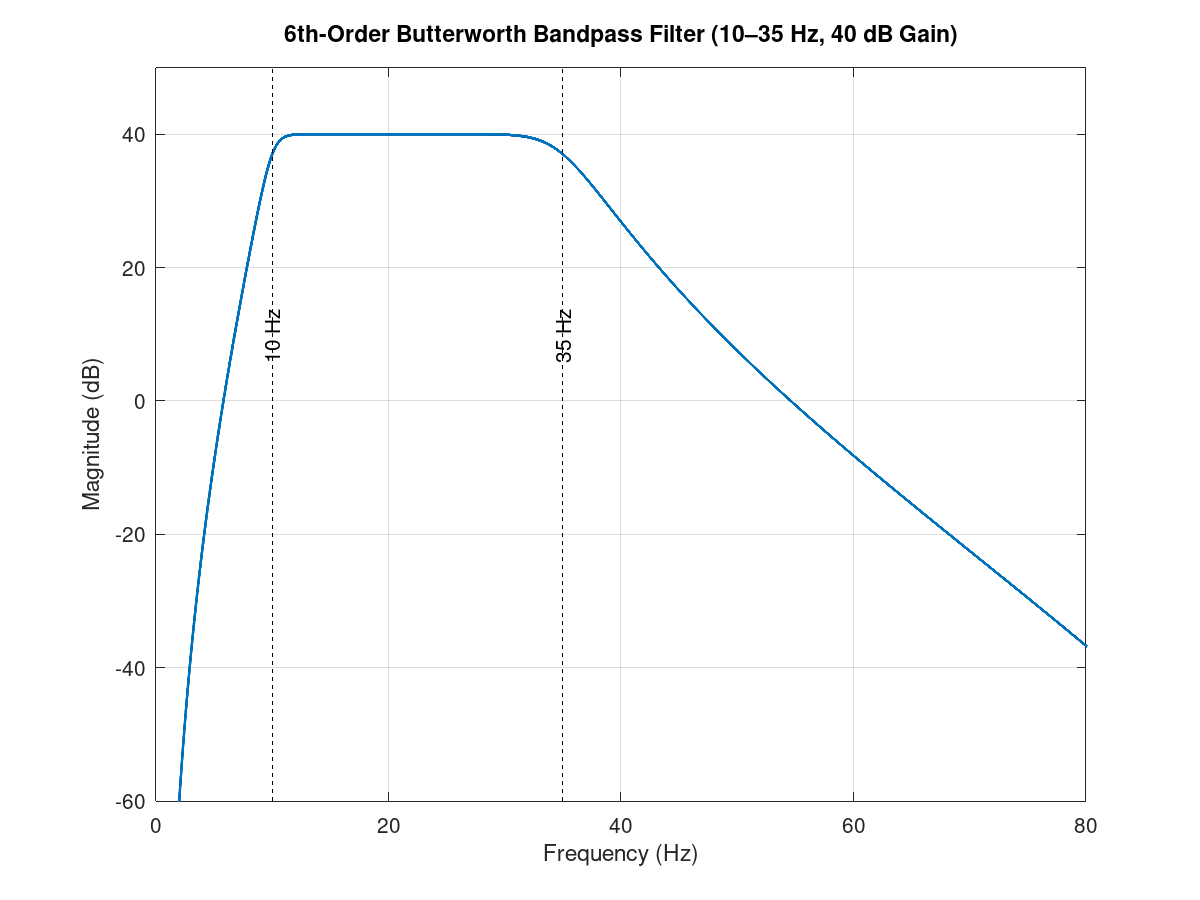
\includegraphics[width=14cm]{src/images/figures/6th_butterworth.png}
	\caption{6th-order Butterworth band pass filter’s frequency response}
	\label{bandpass}
\end{figure}

\section{Microcontroller Based Data Acquisition and Communication}
The microcontroller based data acquisition block will be used to convert the conditioned analog EEG signal to its corresponding digital equivalent which can then be used for real-time processing. The conditioned EEG signal will have the required frequency components after going through the instrumentation amplification and analog filtering blocks, but will still be a continuous time signal. This continuous time signal is fed to the internal ADC of the microcontroller, where the analog signal is converted to its digital counterpart by sampling the signal uniformly with respect to time. Before this process, the signal is level shifted to its mid supply value so that it can be fed to the single supply ADC.

\subsection{Analog to Digital Converter (ADC)}
After the EEG signal is amplified and filtered, it is still an analog signal, meaning it is a continuous voltage that varies with time. However, our microcontroller and signal 
processing algorithms (like FFT) can only work with digital data. Therefore, the signal must be converted from analog to digital, which is done using an Analog to Digital Converter (ADC). 

The filtered EEG signal (in microvolts, now amplified to millivolts/volts) is fed to the ADC input of the microcontroller. The ADC samples the EEG signal at a fixed 
sampling frequency (e.g., 256 Hz or 512 Hz), which is sufficient to capture EEG frequencies (0.5 – 40 Hz). Instead of a continuous waveform, we now have discrete time voltage values. 

The ADC used by our microcontroller is Successive Approximation Register(SAR) ADC. SAR ADC is a type of analog to digital converter that converges digital value towards input signal after every iteration by binary search. Here the search is done by comparing the current digital value in register with input value via DAC and makes a decision to step up or step down the digital value depending on the result of comparision. The digital value is updated from most significant bit to least significant bit. 

\begin{figure}[H]
	\centering
	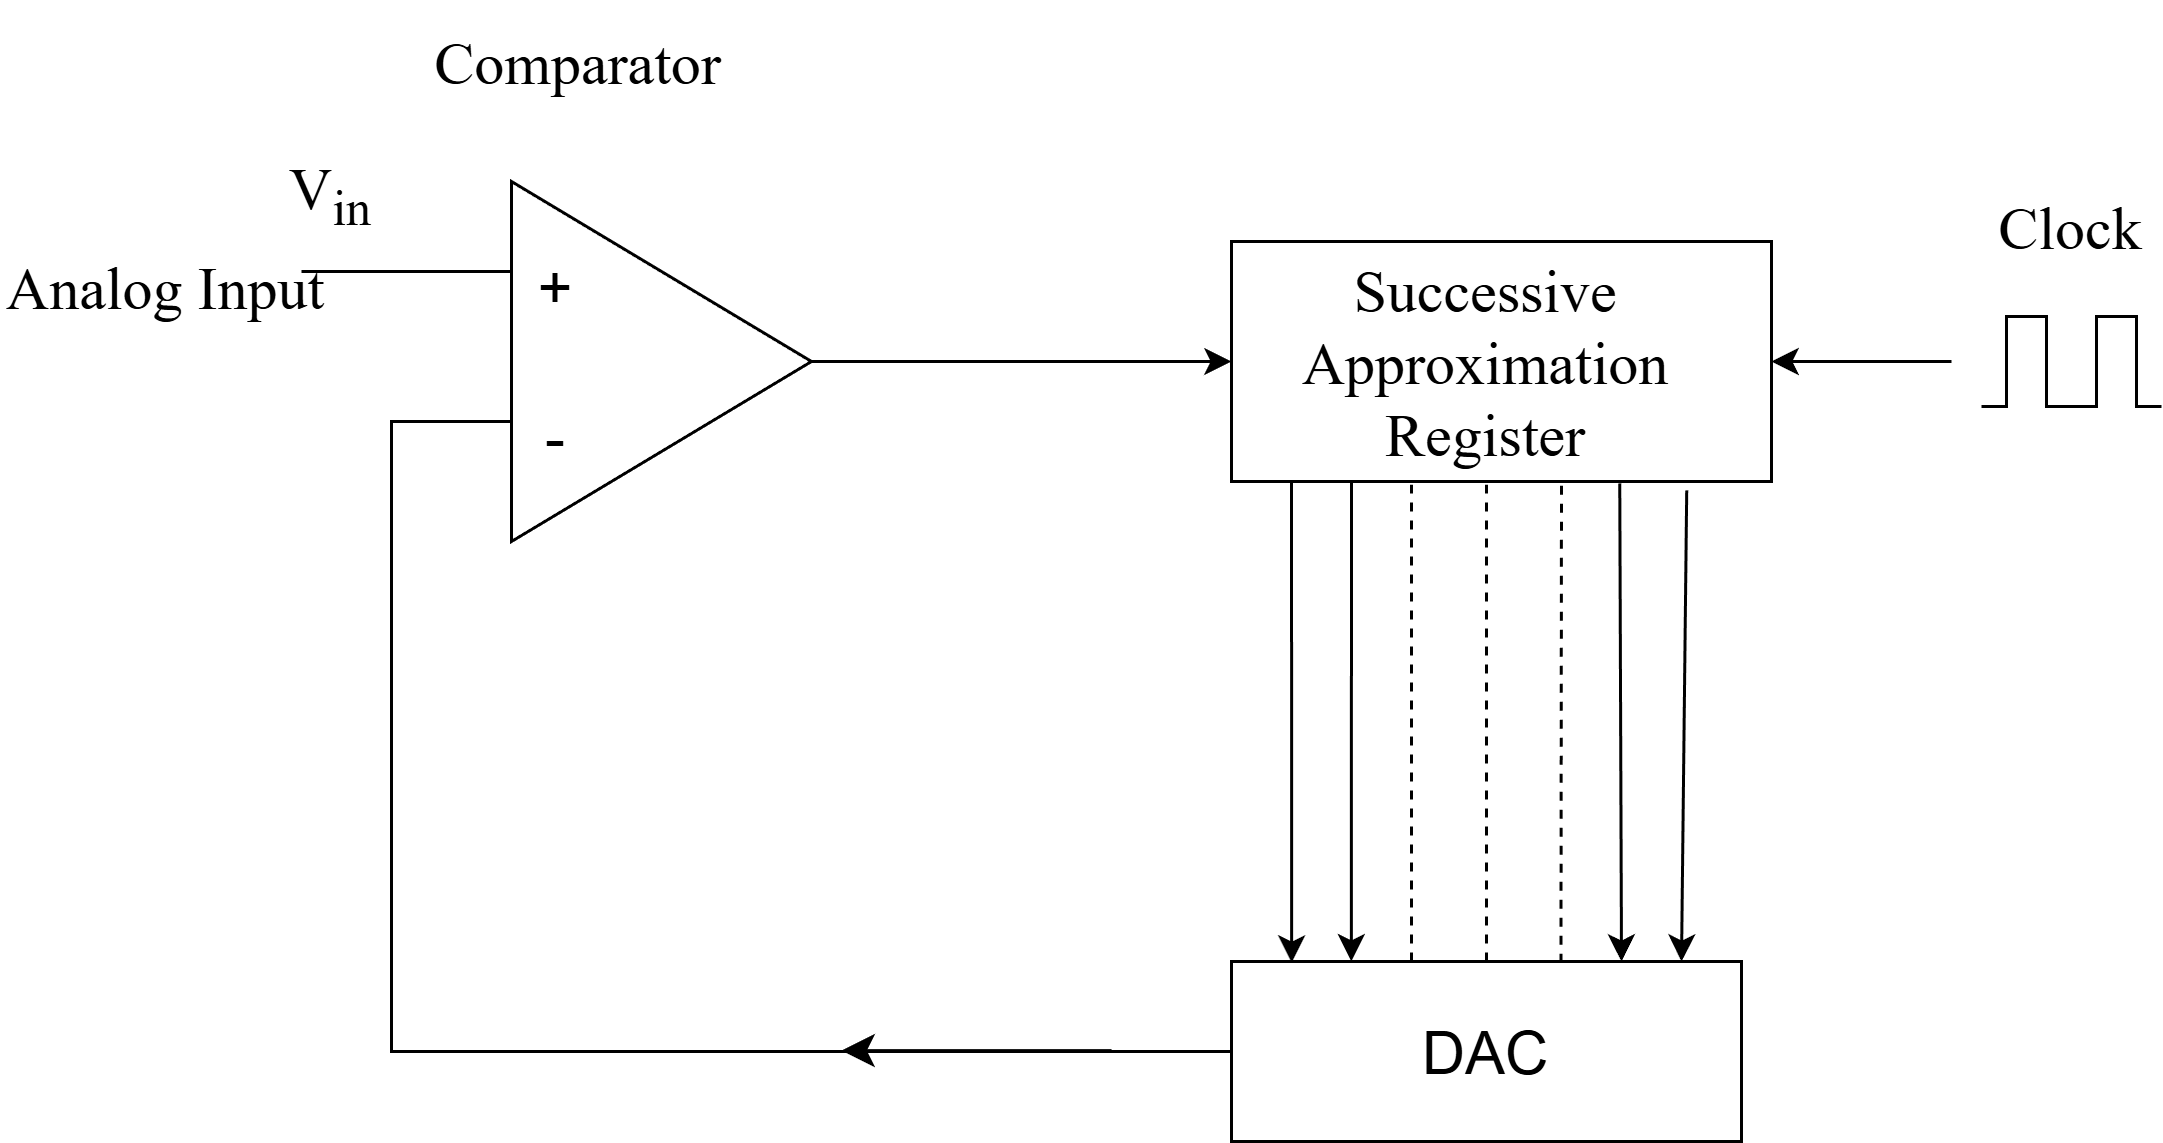
\includegraphics[width = 13.5cm, height=7.5cm]{src/images/figures/sar3.png}
\caption{Successive Approximation Register(SAR) ADC}
\label{Successive Approximation Register(SAR) ADC}
\end{figure}

\section{Arduino Timer Specifications}

Arduino boards, such as the Arduino Uno, feature built-in hardware timers that provide precise time measurement, event counting, and pulse generation. The key specifications of these timers are as follows:

\renewcommand{\labelitemi}{$\bullet$}
\renewcommand{\labelitemii}{$\bullet$}

\begin{itemize}
	\item \textbf{Timer Types:}
	\begin{itemize}
		\item 8-bit timers: Timer0, Timer2
		\item 16-bit timer: Timer1
	\end{itemize}
	
	\item \textbf{Modes of Operation:}
	\begin{itemize}
		\item Normal mode (simple counting)
		\item CTC (Clear Timer on Compare Match) mode
		\item PWM (Pulse Width Modulation) modes
	\end{itemize}
	
	\item \textbf{Clock Source:}  
	Each timer increments based on the system clock (16 MHz on Arduino Uno), optionally divided by a configurable prescaler (1, 8, 64, 256, 1024), allowing flexible timing intervals.
	
	\item \textbf{Interrupt Capabilities:}  
	Timers can generate interrupts on compare match, overflow, or external events, enabling precise periodic execution of code.
	
	\item \textbf{Resolution:}
	\begin{itemize}
		\item 8-bit timers: counts from 0 to 255
		\item 16-bit timer: counts from 0 to 65535
	\end{itemize}
	
	\item \textbf{Applications:}
	\begin{itemize}
		\item Generating precise delays and periodic signals
		\item Measuring time intervals
		\item Counting external pulses or events
		\item Producing PWM signals for motor and LED control
	\end{itemize}
\end{itemize}

\noindent These timers act as hardware counters, providing high accuracy and reliability for time sensitive tasks without relying on software delays.


\section{Frequency Domain Analysis Using Fast Fourier Transform (FFT)}
The digital data is now ready for processing. But the signal is in time domain i.e the signal shows voltage vs time. Brain rhythms (alpha, beta, etc.) are hidden inside the signal. So, the problem is, from the time domain signal alone, we cannot clearly separate brain waves by frequency. For that we need to convert the EEG signals from time domain to frequency domain. And a fourier transform allows us to do that. 
\begin{equation}
	F(\omega) = \int_{-\infty}^{\infty} x(t)\, e^{-j \omega t} \, dt
\end{equation}
where:\\
x(t): The original function or signal in the time domain.\\
$F(\omega)$: The transformed function in the frequency domain.\\
$\omega$: Angular frequency.\\
$e^{-j \omega t}$: A complex exponent representing sinusoidal components.
\section{Discrete Fourier Transform (DFT) and Fast Fourier Transform (FFT)}
The sampled data is discrete, not continuous. And that is why we use discrete fourier transform since the regular fourier transform is for continuous signals. The Discrete Fourier Transform (DFT) is used to convert our discrete time signal from the time domain into its frequency domain representation. It directly computes the frequency components using the DFT formula and requires a large number of computations. For an N point signal, DFT requires $O(N^2)$ complex multiplications, which makes it computationally slow for large data sets.\\The DFT of x[n] is mathematically defined as\\
\begin{equation}
	X[k] = \sum_{n=0}^{N-1} x[n]\; e^{-j \frac{2\pi k n}{N}},\\
	\quad k = 0,1,2,\ldots, N-1
\end{equation}
where,\\
k: index for output frequency component\\
X[k]: the complex frequency domain coefficient corresponding to the k-th frequency\\
N: total number of samples \\
n: the index for sample ranging from 0 to N-1 
x[n]:  n-th sample\\

The Fast Fourier Transform (FFT) is not a different transform but an efficient algorithm used to compute the Discrete Fourier Transform (DFT). FFT exploits the symmetry and periodicity properties of the DFT to reduce the number of calculations. Using FFT, the computational complexity is reduced from $O(N^2)$ to $O(N \log N)$, making it much faster and suitable for real-time signal processing applications such as EEG, ECG, image processing, and communication systems.

The FFT algorithm calculates the frequency components using a computational complexity of $O(N\log N)$, and this makes it possible to process the EEG signals in real-time. The magnitude of the FFT output either $|X[k]|$ or the power spectrum $|X[k]|^2$ shows the magnitude of each frequency component within the EEG signal. Through the power spectrum distribution in different frequency bands, including the beta frequency band (12-30 Hz), one can easily detect whether there are certain brain rhythms within the EEG signals. Therefore, the FFT algorithm converts the time domain EEG signals into frequency domain EEG signals.

\section{CORDIC Algorithm}
As we were implementing FFT algorithm, the need of using sine and cosine trigonometric function became inevitable. Using regular built-in library available is expensive for computation for our 16MHz Arduino micro-controller. So, we decided to adopt CORDIC algorithm to create our custom function which is tuned according to our need of accuracy trading off with the computation as accuracy is disposable since it is not our main concern.

The CORDIC algorithm (COordinate Rotation DIgital Computer) is an efficient iterative method useful to compute various mathematical functions, especially trigonometric, hyperbolic, exponential, logarithmic functions, square roots, and vector rotations using only shift and add operations.


The CORDIC (COordinate Rotation DIgital Computer) algorithm computes vector rotations using only iterative shift-and-add operations. 
A vector $(x, y)$ is rotated by breaking the desired rotation into a sequence of smaller micro-rotations:

\begin{equation}
	\theta_i = \tan^{-1}(2^{-i})
\end{equation}

Each iteration performs a rotation by $\pm \theta_i$, which can be implemented using only arithmetic shifts and additions.

The standard rotation equations are:

\begin{equation}
	x' = x \cos\theta - y \sin\theta
\end{equation}
\begin{equation}
	y' = x \sin\theta + y \cos\theta
\end{equation}

CORDIC rewrites these using the identity $\tan\theta \approx 2^{-i}$, allowing multiplication by powers of two to be replaced with bit shifts.

The iterative update equations become:

\begin{align}
	x_{i+1} &= x_i - d_i \cdot y_i \cdot 2^{-i} \\
	y_{i+1} &= y_i + d_i \cdot x_i \cdot 2^{-i} \\
	z_{i+1} &= z_i - d_i \cdot \tan^{-1}(2^{-i})
\end{align}
where $d_i \in \{-1, +1\}$ determines the direction of rotation.

\subsection{Scaling Factor}

Each micro-rotation introduces a scaling effect on the vector magnitude. After $n$ iterations, the accumulated scale factor is:

\begin{equation}
	K_n = \prod_{i=0}^{n-1} \frac{1}{\sqrt{1 + 2^{-2i}}}
\end{equation}

Thus, the true magnitude must be corrected as:

\begin{equation}
	\begin{bmatrix}
		x_{\text{final}} \\
		y_{\text{final}}
	\end{bmatrix}
	=
	K_n
	\begin{bmatrix}
		x_n \\
		y_n
	\end{bmatrix}
\end{equation}

where $K_n$ is typically precomputed for a given number of iterations.

\section{Twiddle Factor Computation Under Recurrence}
Twiddle factors in the Fast Fourier Transform (FFT) are defined as:

\begin{equation}
	W_N^k = e^{-j \frac{2\pi k}{N}}
\end{equation}

where \(N\) is the FFT size, \(k\) is the index, and \(j = \sqrt{-1}\).

Instead of computing each value using sine and cosine, FFT uses a recurrence approach. Define the general twiddle factor:

\begin{equation}
	W_N = e^{-j \frac{2\pi}{N}}
\end{equation}

Then any twiddle factor can be written as:
\begin{equation}
	W_N^k = (W_N)^k
\end{equation}

From this, we obtain the recurrence relation:
\begin{equation}
	W_N^{k+1} = W_N^k \cdot W_N
\end{equation}

This means each successive twiddle factor is obtained by multiplying the previous one by a fixed complex constant \(W_N\), which corresponds to a constant rotation on the complex unit circle:

\begin{equation}
	e^{j\theta} \cdot e^{j\Delta\theta} = e^{j(\theta + \Delta\theta)}
\end{equation}

Thus:
\begin{equation}
	W \leftarrow W \cdot W_N
\end{equation}

generates all required roots of unity efficiently without recomputing sine and cosine values.

\begin{figure}[H]
	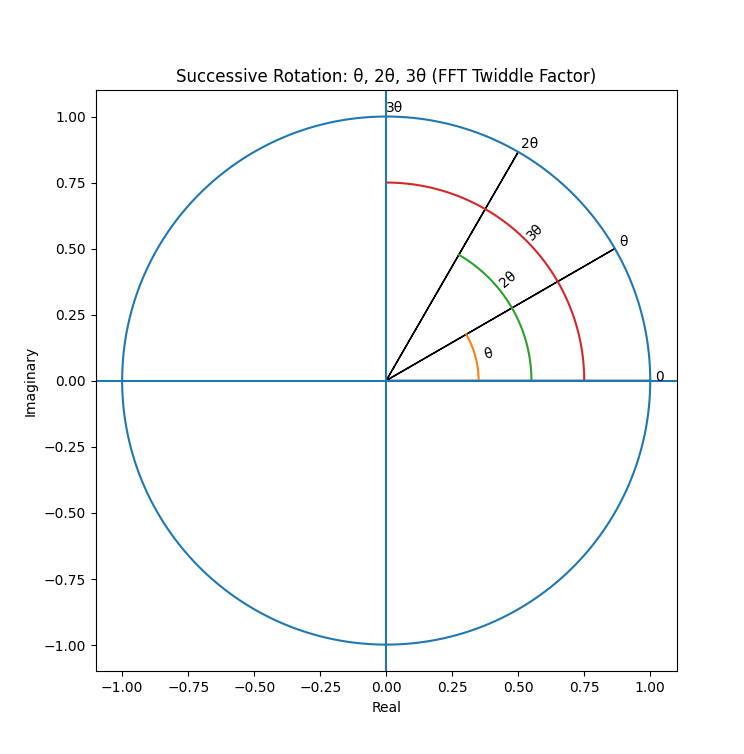
\includegraphics[width=14cm]{src/images/figures/rotation.png}
	\caption{Twiddle Factor Computation Under Unit Circle Rotation}
	\label{twiddle}
\end{figure}


\section{Windowing -- Hann Window}

When performing a Fourier transform, the signal taken for sampling is finite, with no guarantee of perfect start and end points of the waveform, which causes inaccuracies in frequency analysis. Due to this, spectral energy from high-energy frequencies spreads into neighboring frequencies. This phenomenon is known as spectral leakage.

Although spectral leakage cannot be completely eliminated, it can be reduced using windowing techniques. Windowing reduces spectral leakage by smoothing the signal at its boundaries before transforming it from the time domain to the frequency domain.

In this project, the Hann window is used to reduce spectral leakage before transforming the EEG signal. The Hann window smooths abrupt signal transitions by gradually reducing the signal amplitude to zero at the edges, making it suitable for EEG frequency analysis. The Hann window is defined as:
\begin{equation}
w(n) = \frac{1}{2}\left(1 - \cos\left(\frac{2\pi n}{N-1}\right)\right), \quad n = 0, 1, 2, \ldots, N-1
\end{equation}

\begin{figure}[H]
	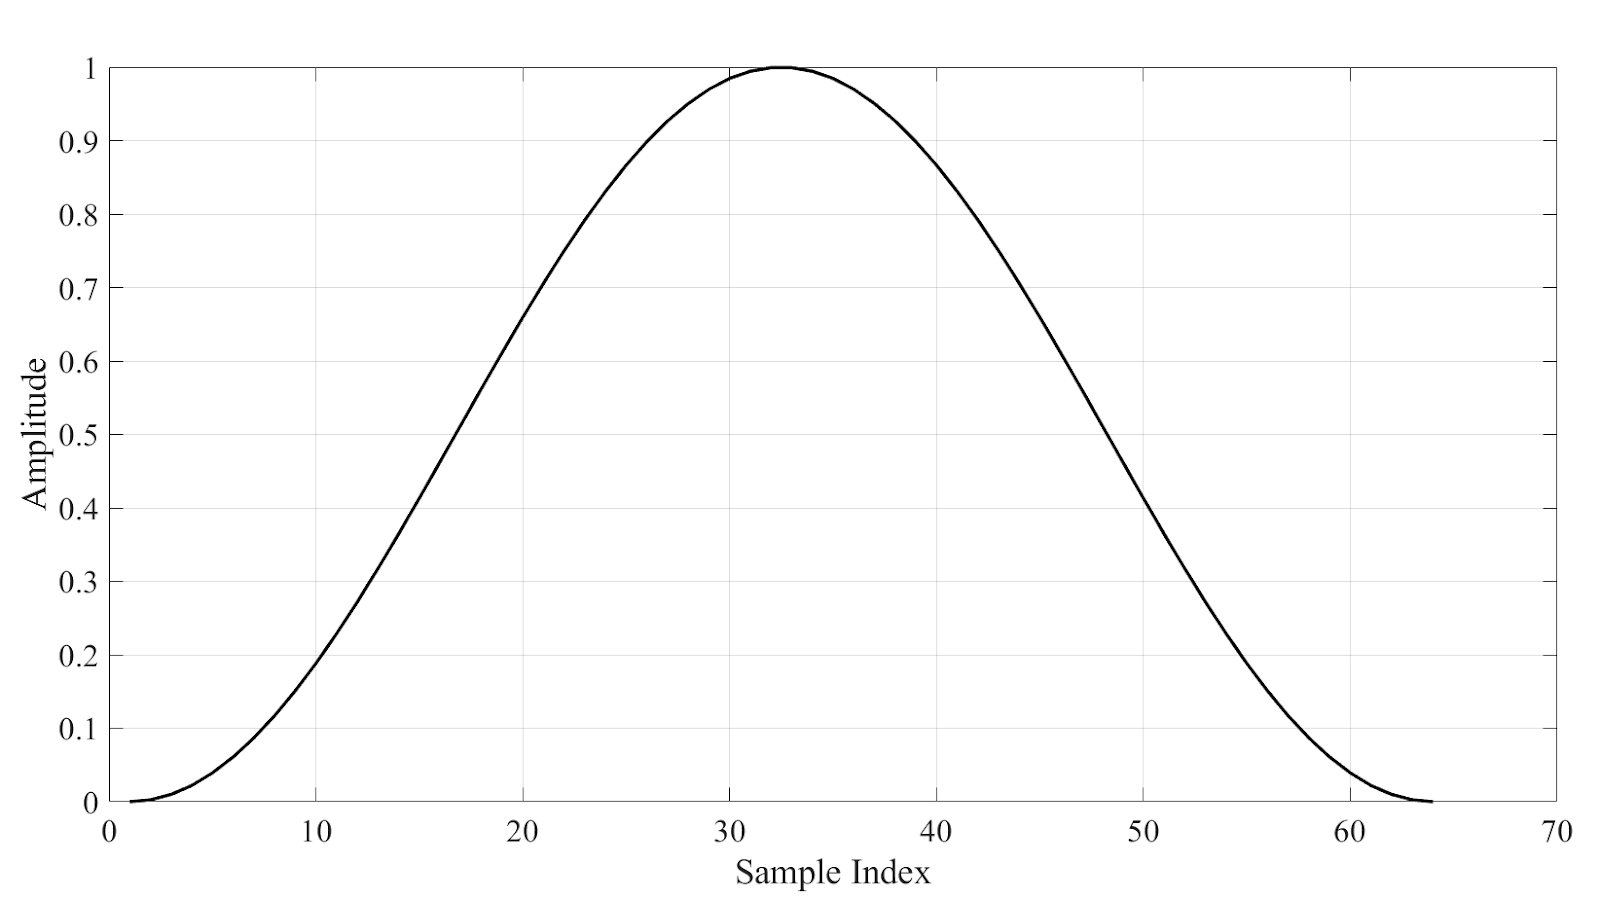
\includegraphics[width=14cm]{src/images/figures/hann.png}
	\caption{Hann Window}
	\label{hann}
\end{figure}

\begin{figure}[H]
	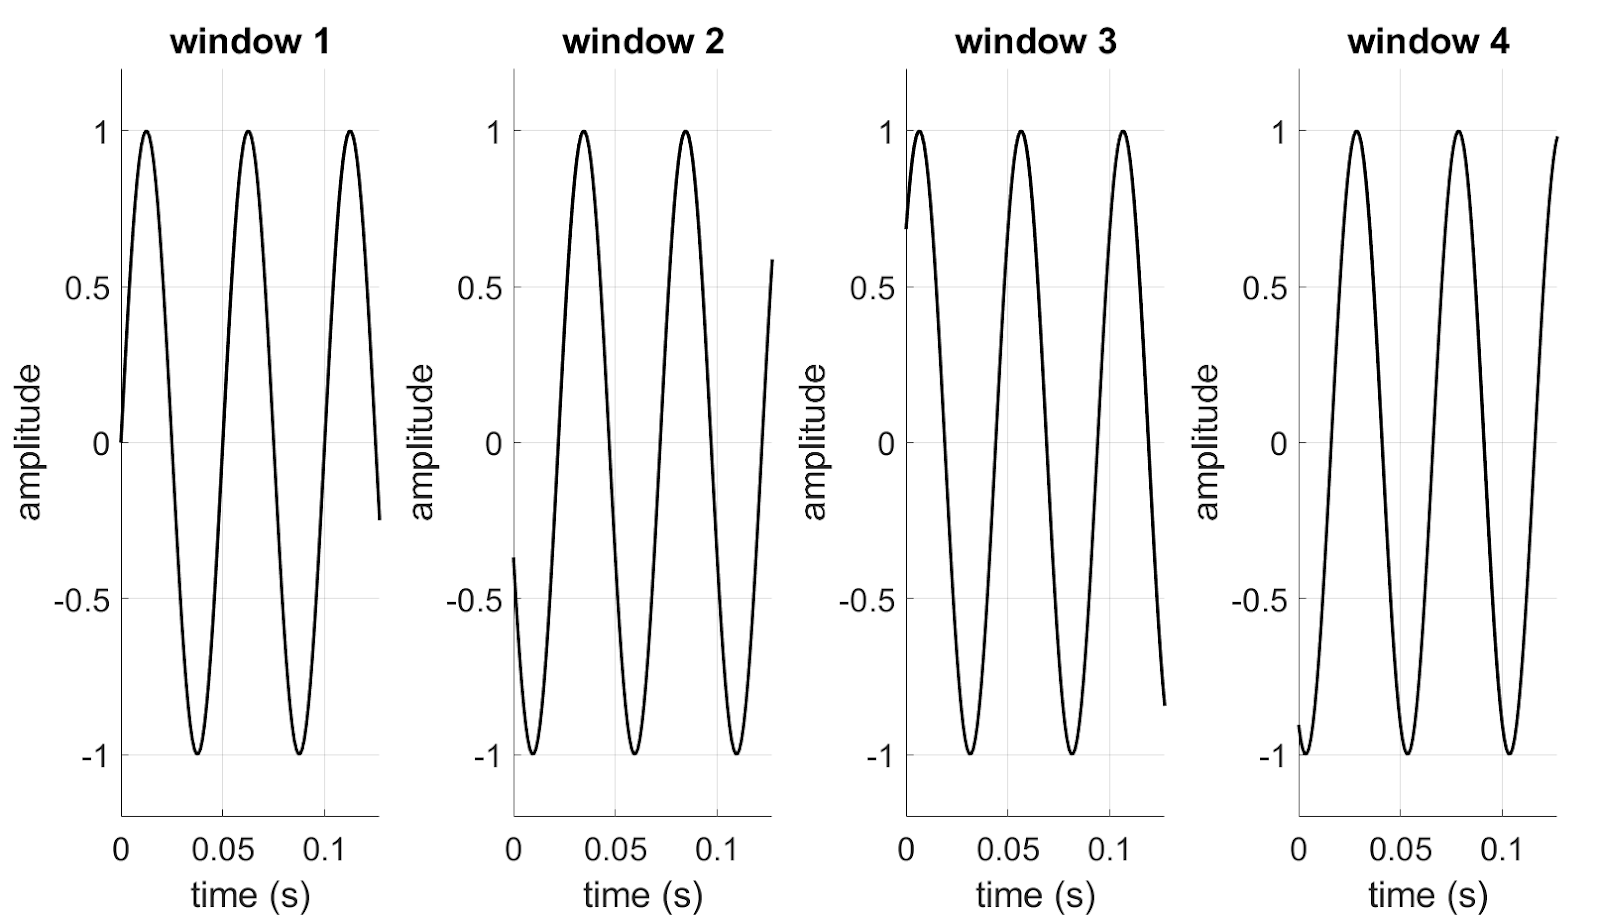
\includegraphics[width=14cm]{src/images/figures/discontinuous_wave.png}
	\caption{Discontinuous wave during window transition}
	\label{discontinuous}
\end{figure}

\begin{figure}[H]
	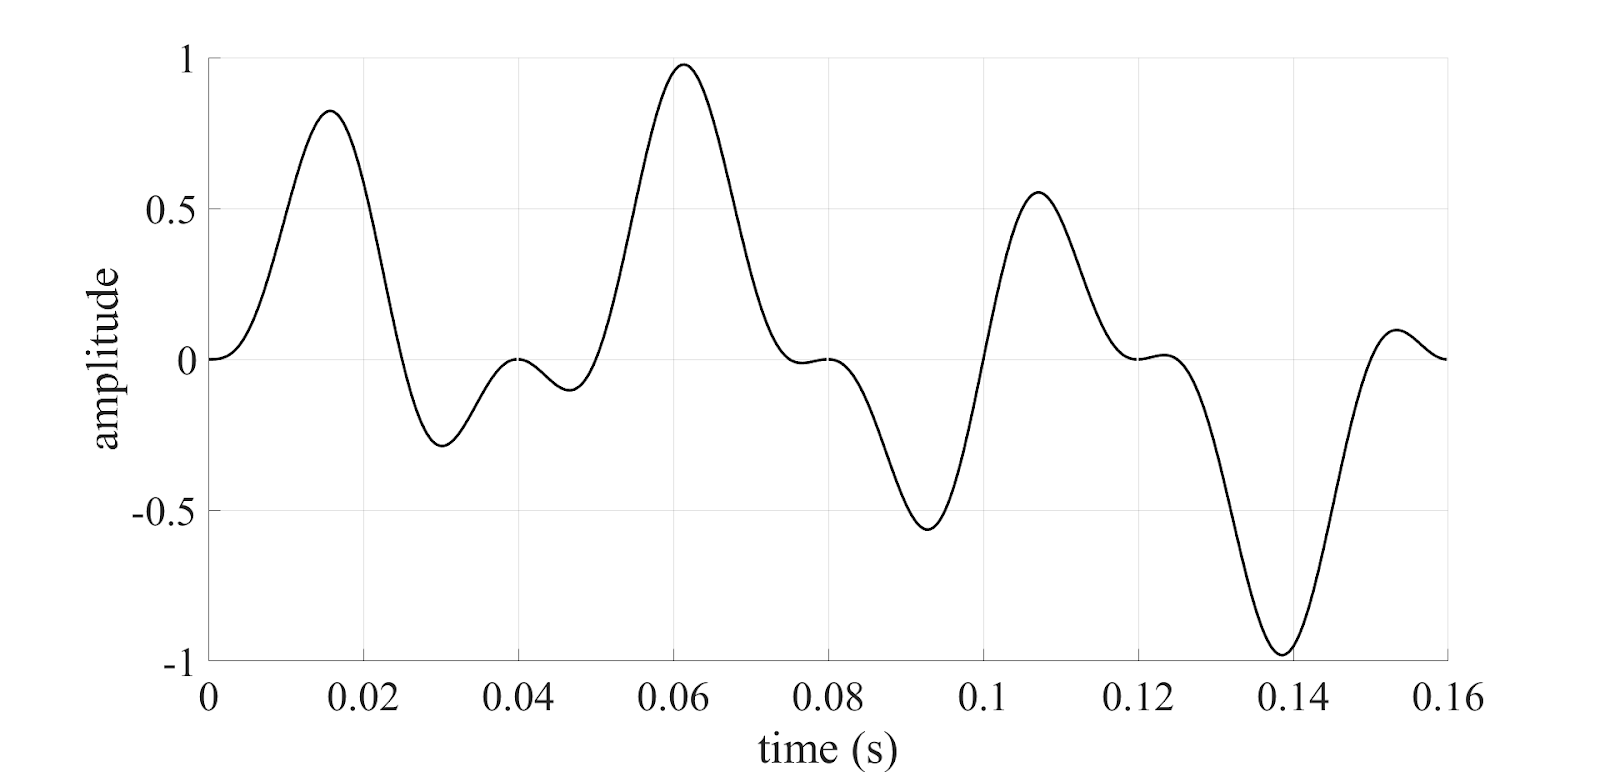
\includegraphics[width=14cm]{src/images/figures/continuity_hann.png}
	\caption{Continuity due to Hann window application on \ref{discontinuous}}
	\label{hann_continuous}
\end{figure}

\section{Processing After Fast Fourier Transform (FFT)}

The output from the Fast Fourier Transform is used to transform the digitized EEG signal from the time domain to the frequency domain. From the output of the Fast Fourier Transform, it is possible to obtain information on the distribution of power in the frequency components of the signal. The power for each frequency is obtained by using the real and imaginary components of the output from the FFT.

The relevant features in the frequency domain are obtained by computing power within certain frequency ranges. Power in the lower frequency range indicates eye blink activity while that in higher frequency ranges such as the beta range (13-30 Hz) indicate focused mental activity. The system uses the computed band-wise power values as its features.

The selected features are compared against pre-defined threshold values in the microcontroller. When the power value for the blink related frequency range exceeds the blink threshold, the system classifies the input signal as eye blink. On the other hand, when the power value for the focus related frequency range exceeds the focus threshold, the system classifies the signal as focus. Accordingly, the system generates commands; blink command for traversing the keys and focus command for key selection.
\chapter{IMPLEMENTATION DETAILS}
\section{Hardware Components}
\subsection{EEG Electrodes}
The basis for operation of EEG electrodes is based on biopotentials. The neural activity within the brain creates electrical potentials due to ions flowing through the membranes of the neurons. These potentials travel across the brain tissue and then to the scalp and skull, creating voltages.

In the experiment, EEG electrodes are placed on the scalp using the international 10-20 system. In the process, a differential method is applied where the voltage potential between the active electrode and the reference electrode is measured. Ground electrode is also used to stabilize the signal.

Blinking of eyes creates high-amplitude and low-frequency signals which are considered electrical artifacts. This is due to the fact that blinking causes eye muscles to contract.

\subsection{Instrumentation Amplifier (AD620)}
AD620 is a high precision instrumentation amplifier which is designed to amplify weak biomedical signals. Due to the nature of the signals generated by the brain, they are very weak and cannot be processed directly.

AD620 achieves amplification by amplifying the difference of two input signals and rejecting any common signal in the two input signals (common mode noise). This feature allows it to reject noise from mains, body movements, and the surrounding environment.
Gain in AD620 can be controlled through an external resistor.

\begin{figure}[H]
	\centering
	
\includegraphics[width = 14.5cm, height=6.5cm]{src/images/figures/instrumentation.png}
	\caption{Instrumentation Amplifier}
	\label{instrumentation}
\end{figure}


\subsection{High Pass Filter}
After instrumentation amplifier, the signals are sent to a highpass filter to remove DC components. This is done in two separate stages: filtering and amplification so that the DC components do not get amplified in the filtering stage.

In the filtering stage, there is unity gain and only high-pass filtering action is performed. The cutoff frequency is:
\[
f_c = \frac{1}{2\pi R_1 C_4}
\]
Substituting the values:
\[
f_c = \frac{1}{2\pi \cdot 3.3\,\text{k}\Omega \cdot 47\,\mu\text{F}} = 1.02\,\text{Hz}
\]

After that, we have a gain stage with gain:
\[
A_v = -\frac{R_4}{R_3}
\]
Substituting the values:
\[
A_v = -\frac{220\,\text{k}\Omega}{5\,\text{k}\Omega} = -44
\]

\begin{figure}[H]
	\centering
	
\includegraphics[width = 14.5cm, height=6.5cm]{src/images/figures/highpass.png}
	\caption{High Pass Filter}
	\label{highpass_filter}
\end{figure}

A small capacitor \(C_5 = 1\,\text{nF}\) is used in this stage, which is important in ensuring the stability of the circuit. It makes sure that there will be no high-frequency noise that can affect the signal and cause oscillation or vibration in the circuit. It can be considered as a kind of shock absorber to keep the signal steady all the time.

\subsection{Signal Amplification}
The first major problem in our project is that brain signals have very low strength. They are usually measured in microvolts, which means they are very tiny.

To make sure that these signals will be readable by a computer, we will use an instrument known as the AD620 Instrumentation Amplifier. Our choice of instrumentation amplifier is because it has the ability to eliminate any common mode noise such as electrical interference from wire and power sources. While other amplifiers add noise to the original signal, the ad620 is a much better option for our purpose.

As for the signal strength needed, we need to control the level of amplification, which is called gain (G).

In AD620, gain is controlled through only one resistor called Rg, connecting Pin 1 and Pin 8.
The formula is:
\[
G = \frac{49.4\,\text{k}\Omega}{R_g} + 1
\]

We decided to use a gain of 16.

Resistor calculation for gain:
\[
G = 16
\]

\[
16 = \frac{49.4}{R_g} + 1
\]

\[
16 - 1 = \frac{49.4}{R_g}
\]

\[
15 = \frac{49.4}{R_g}
\]

\[
R_g = \frac{49.4}{15}
\]

\[
R_g \approx 3.29\,\text{k}\Omega
\]

Since \(3.3\,\text{k}\Omega\) is a standard resistor value, we used \(3.3\,\text{k}\Omega\).

Since we do not apply high gain to boost the signal because it also contains a DC offset that is an unwanted constant voltage that offsets the AC signal. If we apply high gain at the early stages, then it will be large and may lead to saturation where the amplifier cannot accommodate the input anymore and clips the signal. So, we make sure that the initial gain is kept low.

Furthermore, we employ a Driven Right Leg technique, which involves averaging the measured signal and returning a small part of the averaged signal back to the body. The benefit of using this technique is that it helps reduce the common mode noise and interference that may affect the signal quality. Other than reducing noise, the driven right leg helps stabilize the body's reference point for safety purposes. Therefore, the final signal is very clean and free from noise and distortions.

\subsection{Analog Signal Conditioning Using Band Pass Filter}
The analog signal conditioning in the current project is performed using a band pass filter circuit, which serves as an all-in-one solution to the problems of high pass filtering, low pass filtering and rejection of power line interference. The use of a single band pass filter allows to filter out all undesired components and only leave the signal of interest.

The lower cut off frequency of the band pass filter serves as a means of blocking any DC offsets, as well as low frequency components resulting from electrode polarization and head movement. These components carry no useful information about the EEG signal and may impede its further amplification and digitization.

On the other hand, the higher cut off frequency of the band pass filter prevents high frequency noise from entering the system, such as EMG noise produced by muscles of the face and scalp, as well as electromagnetic interference. In order to isolate the brain activity, it is enough to restrict the higher end of the frequency range at 40 Hz.

Moreover, it should be noted that the current design includes a band pass filter, which rejects the component at 50 Hz, thus minimizing the effects of power line interference in the system.

The transfer function is shown below and describes the behavior of the output signal. Transfer function was obtained using nodal analysis, which is a common approach for designing active filters \cite{carter_opamp}. Following is the transfer function of the first stage.

Transfer function first stage:
\begin{equation}
	H_1(s)=\frac{V_o(s)}{V_{in}(s)}
	=\frac{-R_1 C_1\,s}{R_1R_2C_1C_2\,s^2+R_2(C_1+C_2)\,s+1}
\end{equation}

This stage begins removing unwanted signals and keeps the useful brain wave range.


\begin{equation}
	H_1(s)=\frac{-0.03728\,s}{8.0401776\times10^{-5}\,s^2+0.0059487\,s+1}
\end{equation}

\begin{figure}[H]
	\centering
	
\includegraphics[width = 10cm, height=3.5cm]{src/images/figures/filter_first.png}
	\caption{$1^{\text{st}}$ stage band-pass filter}
	\label{filter_first}
\end{figure}

Transfer function second stage:\newline
In this stage, the filter becomes stronger and more accurate. It removes even more unwanted noise using different resistors and capacitors.

\begin{equation}
	H_2(s)=\frac{V_o(s)}{V_{in}(s)}
	=\frac{-R_3 C_3 R_7 \, s}
	{R_3R_4R_7C_3C_4\,s^2+R_4R_7(C_3+C_4)\,s+(R_4+R_7)}
\end{equation}

\begin{figure}[H]
	\centering
	
\includegraphics[width = 10cm, height=3.8cm]{src/images/figures/filter_second.png}
	\caption{$2^{\text{nd}}$stage band-pass filter}
	\label{filter_second}
\end{figure}

\begin{equation}
	H_2(s)=\frac{-1.673\,s}{4.107\,s^2+254.317\,s+87900}
\end{equation}

Transfer function third stage:\newline
This is the final cleanup stage. It works like Stage 2 but uses slightly different values to fine tune the signal. This stage ensures the signal is very clean and ready for use.

\begin{equation}
	H_3(s)=\frac{V_o(s)}{V_{in}(s)}
	=\frac{-R_5 C_5 R_8\,s}
	{R_5R_6R_8C_5C_6\,s^2+R_6R_8(C_5+C_6)\,s+(R_6+R_8)}
\end{equation}

\begin{figure}[H]
	\centering
	
\includegraphics[width = 10cm, height=3.8cm]{src/images/figures/filter_third.png}
	\caption{$3^{\text{rd}}$stage band-pass filter}
	\label{filter_third}
\end{figure}

\begin{equation}
	H_3(s)=\frac{-3.40331\,s}{14.4350344\,s^2+516.864\,s+103300}
\end{equation}

Final transfer function:
\begin{equation}
	H(s)=H_1(s)H_2(s)H_3(s)
\end{equation}

\begin{align}
	H(s) &=
	\frac{(-0.03728s)(-1.673s)(-3.40331s)}
	{(8.040\times10^{-5}s^2+0.0059487s+1)
		(4.107s^2+254.317s+87900)} \notag \\
	&\quad \times
	\frac{1}
	{(14.435s^2+516.864s+103300)}
\end{align}

\begin{figure}[H]
	\centering
	
\includegraphics[width = 14.5cm, height=6.5cm]{src/images/figures/three_stage.png}
	\caption{Three-stage $6^{\text{th}}$-order band-pass filter}
	\label{three_stage}
\end{figure}


\subsection{Arduino Microcontroller (ADC \& Control Unit)}
The role of the Arduino is to serve as an interface between the analog EEG hardware and the computer. This is because the Arduino board comes with an integrated analog to digital converter (ADC) that converts the conditioned analog signals into digital information.

The ADC measures the input voltage periodically and translates it into a numeric value depending on the reference voltage and ADC resolution (normally 10 bits). The resulting digital signal can be manipulated through software. Subsequent to this conversion, the Arduino transfers the information to the computer using the USB serial connection (internally uses the UART protocol).

\subsection{Timer1 - Arduino}
The Timer1 of arduino is configured in CTC mode to generate interrupts at a rate of 1024 Hz. This allows the Arduino to sample the analog input at at desired intervals and independant of the main program. The configuration details are:

\begin{itemize}
	\item {Timer:} Timer1 (16-bit)
	\item {Mode:} CTC (Clear Timer on Compare Match)
	\item {Prescaler:} 1
	\item {Compare Register (OCR1A):} 31249
	\item {Interrupt Frequency:} 
	\[
	f_\text{interrupt} = \frac{f_\text{CPU}}{(OCR1A + 1) \times \text{Prescaler}} 
	= \frac{16\,\text{MHz}}{31249 \times 1} = 512~\text{Hz}
	\]
\end{itemize}

\noindent The ISR reads the analog input and stores it in a double buffer for further processing:

\subsection{Interconnection of Hardware Components}
All hardware devices are interconnected to develop an effective EEG-based BCI system. Signals from the brain along with eye blink activity are recorded using EEG electrodes and are amplified using the AD620 instrumentation amplifier. Amplified signals are filtered using the bandpass filter in order to eliminate the noise.

The filtered signal is then digitized using the ADC feature of the Arduino microcontroller. The digital signal is transferred to MATLAB using the serial port. Signal processing is done in MATLAB using FFT and time domain analysis for the detection of eye blinks and brain waves activity. According to the set threshold values, control commands are generated using rules and are mapped to simple text entry device.

This hardware-software combination proves to be an effective and economical example of BCI system.

\section{Software Components}
\subsection{Arduino Firmware}
The Arduino firmware serves as the data acquisition and communication interface of the project. Its main purpose is to continuously acquire the filtered EEG signal from the analog input pin via the built-in Analog to Digital Converter (ADC) of the board and send it to the computer.

The ADC of the Arduino digitizes the incoming analog EEG signal using the board's reference voltage and ADC resolution. In the present project, the amplified and filtered EEG signal falls within the safe operating limits of the Arduino's ADC. The firmware is written in such a way as to acquire the signal at a fixed and constant sampling frequency to enable frequency domain analysis using FFT in MATLAB.

The sampling period of the ADC can be achieved through the use of a timer or delay function in the firmware code. The acquired samples are transmitted in real-time to the computer via the USB serial communication protocol, which uses the UART interface. The baud rate of the USB serial connection is chosen to enable lossless real-time data transfer.

The Arduino firmware does not do any complex signal processing. It is only responsible for data acquisition and real time transmission of the acquired data. All other processing tasks are done using MATLAB.
Functions in the Project:
\begin{itemize}
	\item To read analog EEG signal using Arduino ADC
	\item Maintain constant sampling frequency
	\item Convert analog voltage into corresponding digital values
	\item Send the digital data to MATLAB via USB serial link
\end{itemize}


\subsection{MATPLOTLIB}
Python is used as the platform for signal processing, analysis, and visualization in the proposed project. Real time EEG data sent via serial port from Arduino microcontroller is processed in Python using digital signal processing techniques. Various Python libraries like NumPy, SciPy and Matplotlib are used for computing, frequency analysis and graphical visualization respectively.

Initially, the acquired EEG samples are plotted in the time domain using the Matplotlib library. The eye blink events can be identified as high amplitude peaks in the time domain waveform. The Python program continuously checks the amplitude value of the received signal and uses a threshold-based algorithm to detect eye blinks in real time.

The frequency analysis of brain waves requires the signal to be segmented into short time segments of equal duration. Each time segment is subjected to a Hann window before performing the Fast Fourier Transform (FFT) in order to reduce spectral leakage. The NumPy and SciPy libraries are used to compute FFT in order to convert the EEG signal from time domain to frequency domain.

In this experiment, we are interested in analyzing the beta waves which lie in the frequency band between 12 Hz to 30 Hz. The Python program computes the spectral power in this frequency band and compares it with the pre-defined threshold to estimate the user's mental state like relaxed or focused.

Eye blink detection and beta wave detection are considered as the features in the project. Eye blink detection serves as a control/selection function while beta wave detection serves as a decision factor. Rule based decision algorithm generates command to the text selection interface based on the detections mentioned above. The results and plots are displayed using Matplotlib library showing a human-computer interaction system driven by brain signals.


\section{Calibration Process of Each Module}
\subsection{EEG Electrode Calibration}
\begin{itemize}
	\item Skin preparation is carried out to minimize impedance between electrodes
	\item Electrodes are tightly fixed to minimize movement and provide stable contact
	\item Baseline brain waves are collected to confirm the availability of the EEG signal
\end{itemize}

\subsection{Amplifier Calibration}
\begin{itemize}
	\item The gain of AD620 amplifier is set using external resistors
	\item Output response is evaluated using low amplitude input signals
	\item Offset voltage is checked to avoid saturation of signals
\end{itemize}

\subsection{Filter Calibration}
\begin{itemize}
	\item High and low pass cutoff frequencies are checked
	\item Filter frequency response is measured using signal generators
\end{itemize}

\subsection{ADC Calibration}
\begin{itemize}
	\item Reference voltage for Arduino ADC is confirmed
	\item Input signal range is checked to avoid clipping
	\item Sampling frequency is evaluated for accurate FFT
\end{itemize}




\section{Interfacing Technicalities and Protocols}
\subsection{EEG Electrodes to Amplifier Interface}
The interfacing of the EEG electrodes with the instrumentation amplifier occurs through the use of differential connection techniques. Here, two active electrodes are employed to detect the voltage difference produced by brain activity with a reference electrode for comparison purposes. The ground electrode acts as the common reference point of the system where it is connected to the body of the subject under study. This is necessary since EEG signals are very small in magnitude and easily susceptible to interference.

Shielding of the wires connecting the electrodes to the amplifier inputs is done to prevent any form of electromagnetic interference from other electrical devices. Appropriate skin preparation and tight electrode attachment are critical in minimizing the electrode-skin impedance. This ensures that no distortion of the signal occurs. The differential connection technique enables the amplifier to accurately pick the EEG signals and artifacts caused by eye blinks.

\subsection{Amplifier to Filter Circuit Interface}
The output from the AD620 instrumentation amplifier is connected directly to the input of the analog filter circuit. Signal matching is vital at this point since the amplified signal must stay within the operational range of the filter circuit components. Gain adjustment of the amplifier is carried out to make sure that the amplified signal is large enough for filtering purposes without saturating the filter circuitry.

Grounding techniques are applied to eliminate possible ground loops which could lead to more noise and system instability. Both amplifier and filter circuits have a common ground to ensure signal integrity. Connecting the amplifier output directly to the filter input makes sure that signal flow is uninterrupted throughout this part of the process and undesired frequencies are eliminated.

\subsection{Filter to Arduino Interface}
After the analog conditioning of the signal, the filtered EEG signal will be connected to the Arduino microcontroller using an analog input pin on the microcontroller. Because the analog to digital converter (ADC) used in the microcontroller cannot take input voltages greater than 5 volts, it is ensured that the filtered output voltage stays below this maximum level.

The filtered output signal corresponds to the clean EEG signal which contains brain activities and eye blink events. This signal is fed to the analog input pin of the microcontroller where it is sampled at equal intervals. The ground connection between the filter circuit and the microcontroller remains common for both of them.
\subsection{Fast Fourier Transform}
FFT is used to analyze the frequency components of the signal.The pseudocoe for the implementation of FFT is given below:

\begin{algorithm}[H]
	\caption{Cooley-Tukey FFT}
	\label{alg:fft}
	\begin{algorithmic}[1]
		\Require $x[0..N-1]$: sequence of sample, $N$ a power of 2
		\Ensure $X[0..N-1]$: discrete Fourier transform of $x$
		\If{$N = 1$}
		\State $X[0] \gets x[0]$
		\Else
		\State $x_\text{even} \gets x[0], x[2], \dots, x[N-2]$
		\State $x_\text{odd} \gets x[1], x[3], \dots, x[N-1]$
		\State $X_\text{even} \gets \text{FFT}(x_\text{even})$
		\State $X_\text{odd} \gets \text{FFT}(x_\text{odd})$
		\For{$k = 0$ to $N/2 - 1$}
		\State $t \gets X_\text{odd}[k] \cdot e^{-2 \pi i k / N}$
		\State $X[k] \gets X_\text{even}[k] + t$
		\State $X[k + N/2] \gets X_\text{even}[k] - t$
		\EndFor
		\EndIf
		\State \Return $X$
	\end{algorithmic}
\end{algorithm}

\textbf{Bit Reversal}\newline
The bit reversal technique is a preprocessing step used in the Cooley-Tukey Fast Fourier Transform (FFT) to enable in place computation and reduce memory usage. In the FFT, the input sequence is recursively divided into even and odd indexed elements. This recursion can consume extra memory due to multiple temporary arrays.

We can reorder the sample sequence to perform the computation with low memory cost using bit reversal by reversing bits. For our use 1 byte memory is more than enough for bit reversal so we have put in pre defined array as 64 sized array is enough for this computation. After reordering, the FFT algorithm can operate iteratively and in place, eliminating the need for recursive subarrays. This reduces memory overhead, improves cache efficiency, and allows the FFT to maintain its computational complexity of $N \log N$.

An N point signal is decomposed into N signals each containing a single point.
Each stage uses an interlace decomposition, separating the even and odd numbered samples.
\begin{figure}[H]
	\centering
	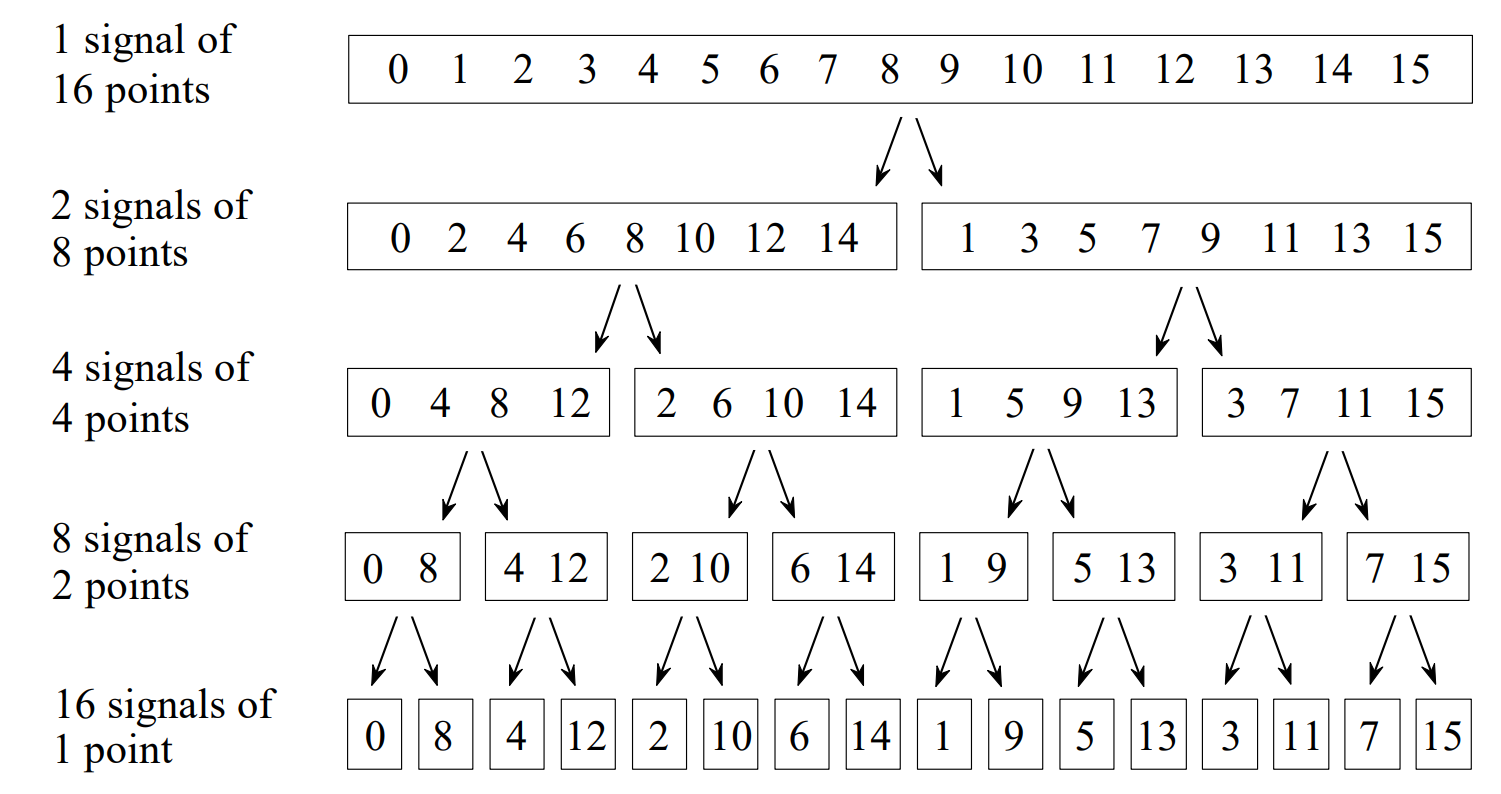
\includegraphics[width = \textwidth, height=7cm]{src/images/figures/odd_even.png}
	\caption{The FFT sample decomposition. \cite{smith1999dsp}
	}
	\label{odd_even}
\end{figure}

\begin{table}[H]
	\centering
	\caption{Bit-reversal permutation for $N=8$ FFT}
	\label{tab:bitreversal}
	\begin{tabular}{c c c c}
		\hline
		\textbf{Original Index} & \textbf{Binary} & \textbf{Reversed Binary} & \textbf{Bit-Reversed} \\ 
		\hline  % thinner line between header and data
		0 & 000 & 000 & 0 \\
		1 & 001 & 100 & 4 \\
		2 & 010 & 010 & 2 \\
		3 & 011 & 110 & 6 \\
		4 & 100 & 001 & 1 \\
		5 & 101 & 101 & 5 \\
		6 & 110 & 011 & 3 \\
		7 & 111 & 111 & 7 \\
		\hline
	\end{tabular}
\end{table}

\subsection{Arduino to MATLAB Communication Interface}
Data transfer between the Arduino and the MATLAB is performed via USB-based serial communication, where the internal protocol used by the USB-based serial communication is UART (Universal Asynchronous Receiver Transmitter). Arduino sends the digitized data from the EEG sample to the computer in the form of serial packets.

Baud rate for the serial communication is chosen appropriately such that there is no loss or corruption of the transmitted data due to the high speed of transfer. The MATLAB opens a serial port to receive the data packet, synchronizes with the Arduino, and performs real-time processing on the received samples.




\chapter{RESULTS AND ANALYSIS}

\section{EEG Signal Acquisition Result}
Signals with lower amplitudes in the microvolt level were fed to the input of the instrumentation amplifier in order to simulate EEG signals. The signal at the output of the instrumentation amplifier designed using the AD620 showed no signs of distortion. The output signal proved to be stable enough to be processed in the next steps.
Thus, the amplification stage has shown itself to be effective enough to amplify low-level biopotential signals.

\section{High Pass Filter}
 
\begin{figure}[H]
	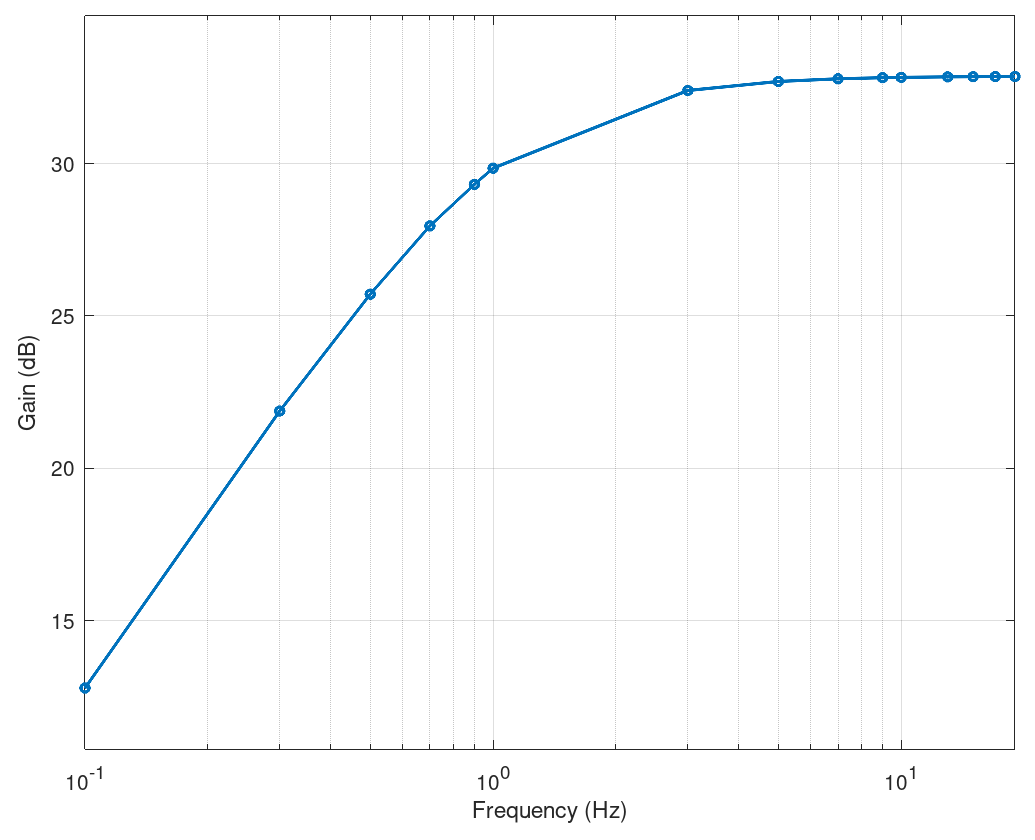
\includegraphics[width=\textwidth]{src/images/figures/highpass_plot.png}
	\caption{Bode plot of High Pass Filter's frequency response}
	\label{frequency_response_highpass}
\end{figure}

\section{Band Pass Filter}
\begin{figure}[H]
	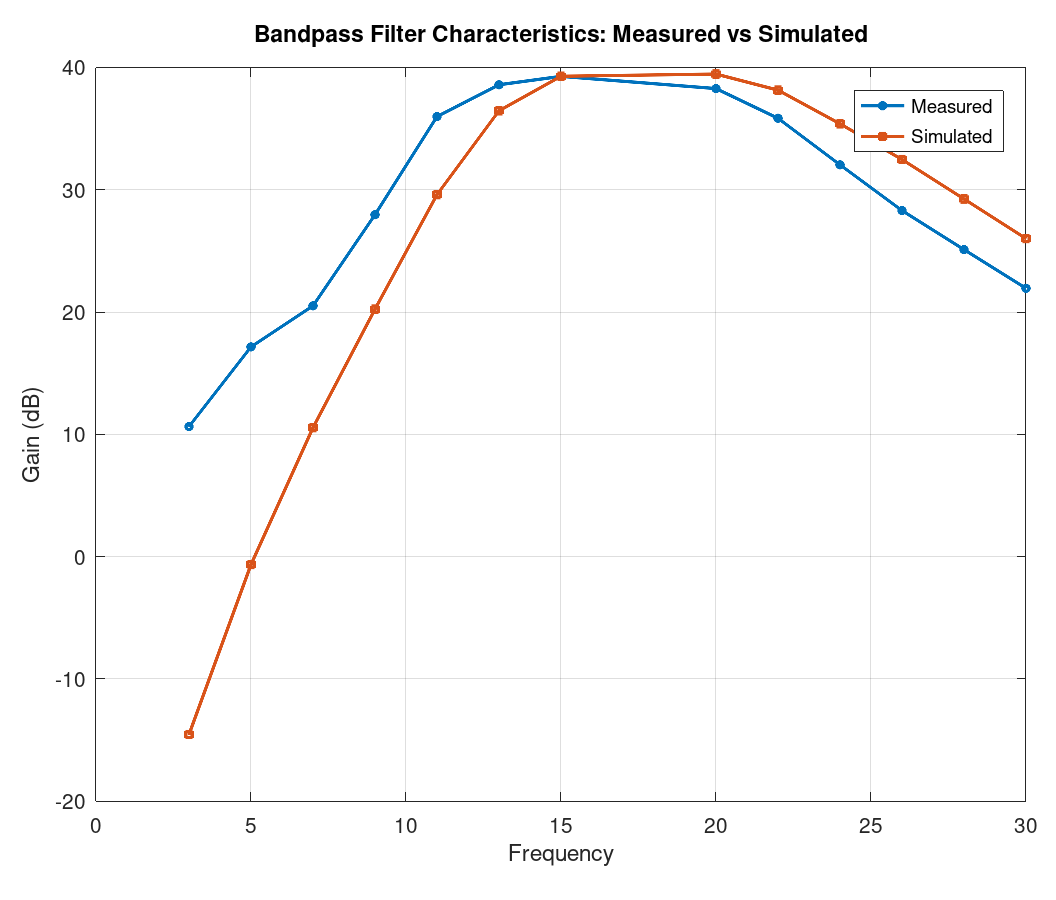
\includegraphics[width=\textwidth]{src/images/figures/bandpass_compare.png}
	\caption{Frequency Response of Band Pass Filter}
	\label{bandpass_compare}
\end{figure}

\section{FFT of Recieved Signal}
\begin{figure}[H]
	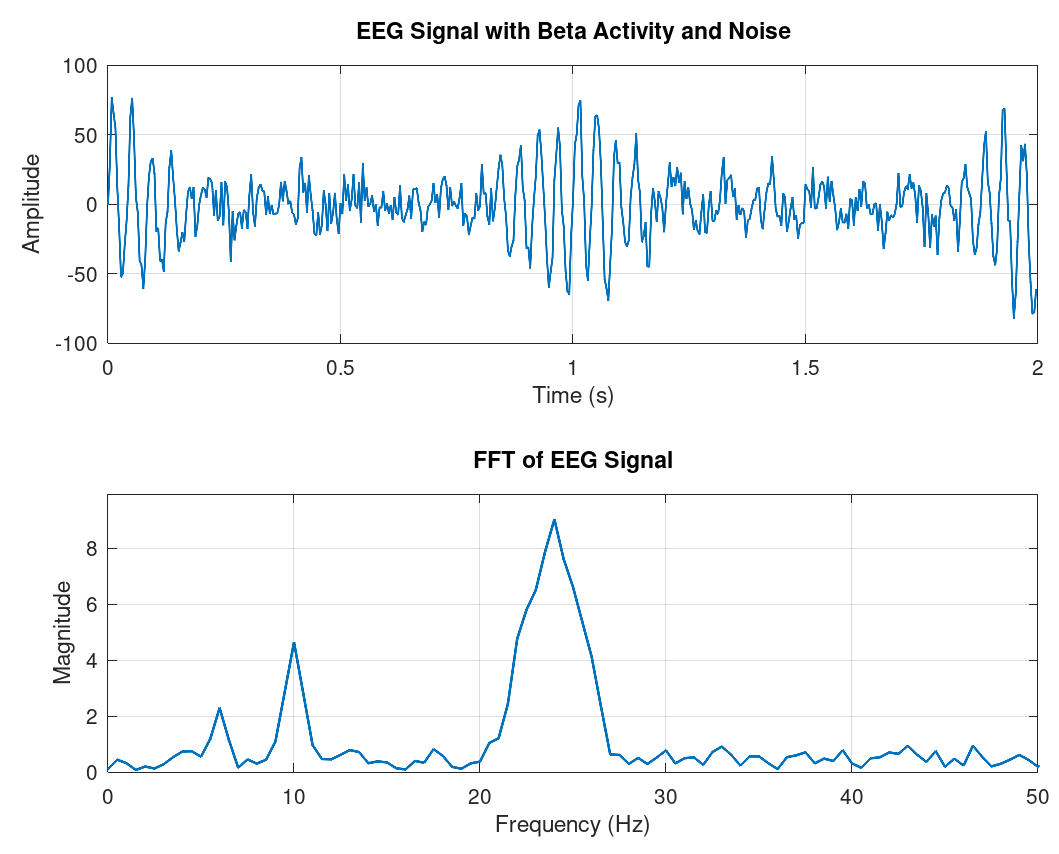
\includegraphics[width=\textwidth]{src/images/figures/betawaves.png}
	\caption{FFT plot of recieved signal}
	\label{betawaves}
\end{figure}

The filtered signal showed significant reduction in noise components, resulting in a cleaner waveform suitable for frequency analysis.

\section{Frequency Domain Analysis Using FFT}
FFT was used on the filtered signal in order to transform the signal from the time domain into the frequency domain. The FFT result showed prominent frequency peaks representing the frequency of the input signal from the function generator.

Upon setting the input signal frequency in the beta band range (12-30 Hz), a pronounced peak was seen in the FFT graph in the beta band range. This proves that the system can detect certain EEG frequency bands using frequency domain analysis.

\section{Confusion Matrix}
\begin{figure}[H]
	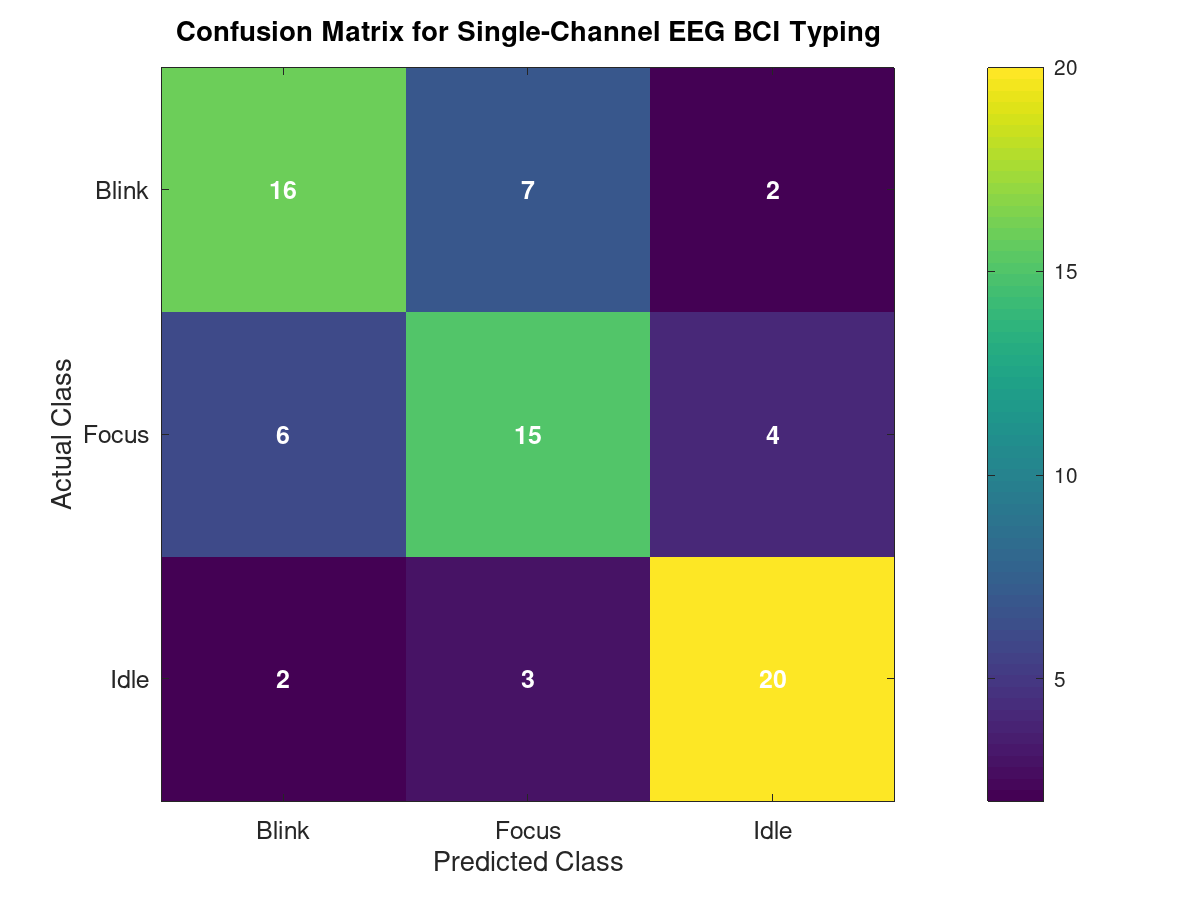
\includegraphics[width=\textwidth]{src/images/figures/confusion.png}
	\caption{Confusion Matrix}
	\label{confusion}
\end{figure}

This confusion matrix was used to analyze the classification ability of single-channel EEG-based BCI typing system in distinguishing three states: blink, focus and idle. Rows correspond to the actual classes, whereas columns denote the classes assigned by the system. The numbers along the diagonal represent the correct classifications. In other words, the system identified 16 blinks, 15 focuses and 20 idles out of 25 trials of each class respectively. Thus, the total accuracy equals to 68\%. These results prove that the system is capable of detecting user intentions at the most general level. Nevertheless, it should be noted that the performance was different for each particular class.

One may observe the main issue represented in the confusion matrix, namely the confusion between blink and focus. More specifically, there were 7 cases when blink was identified as focus and 6 cases when focus was confused with blink. In other words, these types of mistakes comprised the major source of errors in the system. One of the reasons behind this problem was that blink and focus were measured from the same channel of EEG. The fact that only one channel was used made it rather difficult to distinguish between two types of activity. A blink usually causes significant signal shift, however, focus may also lead to such changes, particularly if the user makes some slight movements with eyes, changes forehead tension and produces muscular activity while concentrating. Consequently, the system managed to understand that some intentional activity occurred, but failed to determine whether it was blink or focus.

As for the results achieved for the idle class, they were rather good, i.e. 20 correct identifications out of 25. This may be explained by the fact that idle state is more stable and close to the baseline signal than other two types of activity. Nevertheless, several cases of incorrect classification were also observed for this type. They might be caused by noise, unintentional movements of eyes and some signal shifts which had nothing in common with any commands. As for the worst results obtained for focus, they are quite understandable. It is much easier to identify blink than focus since blink lasts for a rather short period, whereas focus refers to some kind of mental state changing very slowly.



%\chapter{FUTURE ENHANCEMENTS}

Many options exist for future improvements that will enhance the accuracy, speed, and usefulness of the BCI system. This is because the current system operates as a mere prototype with lots of limitations in terms of the hardware used and the way the signals have been processed. Improvements could be made by enhancing the circuitry, having more input channels, improved classification techniques, and realistic typing interface.

\section{Hardware Improvements}

The first possible improvement in the future would be to redesign the circuit in a proper printed circuit board instead of using a matrix board. It would decrease noise and improve connections, increasing the reliability of the system. Moreover, better shielding and grounding can be used to minimize the interference caused by the power lines and other electronic devices. The DRL circuit can also be improved with adjustable gain using a potentiometer in order to adjust noise cancellation for proper testing. Better electrodes and electrode placement will also help to collect cleaner signals.

Secondly, an increase in number of EEG channels will be a major improvement in the future. Currently the system uses only one channel to detect blinks and focus at the same time. Therefore, using more channels will provide more data about the brain and its functions, allowing to classify signals more accurately. Moreover, more channels will also allow to compare the signals across all the electrodes rather than focusing on one path, reducing confusion between blink, focus and idle states. Consequently, more complicated commands can be developed for BCI systems in the future.

\section{Signal Processing Improvements}

The signal processing stage is also open to further improvements in several aspects. The use of superior methods for digital filtering could help eliminate noise and artifacts more efficiently. Given that the current device operates within a restricted frequency band, future implementations could extend their research into other EEG bands and examine their utility in the focus determination process. In addition, better artifact removal techniques could be employed to improve the ability to deal with ocular movement noise, muscle activity and power-line interference.

A great idea for an improvement would be to perform some signal processing operations, including FFT and feature extraction, on a more powerful platform than Arduino. Considering that the use of such operations with the current processor has some limitations, using a more efficient processor could help achieve better results in analyzing the brain signals. Better sampling qualities and resolution could lead to increased accuracy in detecting small changes in the EEG signal.

\section{Classification and Machine Learning Improvements}

The present system seems to employ a relatively simple approach to classify blink, focus and idle states, however in the future more sophisticated approaches can be employed. For instance, such features of EEG signal as amplitude, band power, energy, variance or time frequency representation can be extracted and provided as input data for classification algorithms such as support vector machines, k-nearest neighbors, decision trees or neural networks.

Machine learning can also allow the system to adapt to specific user. Indeed, as EEG signals vary from person to person, a model developed for one particular user cannot necessarily be used for another person. In the future, the system can incorporate user calibration and training to adapt to a particular user. Also, the system can use adaptive threshold or even online learning to ensure more consistent performance across different sessions.

\section{Interface and functionality improvements}

Even the typing interface itself can be enhanced in further research. At present, only a basic BCI can be created as the system recognizes only a few signals. However, with improved classification and additional channels, extra functions may be introduced, such as select, delete, move left, move right, confirm or switching between different keyboard groups. These additional functions will provide a user with greater flexibility in terms of typing. In addition, predictive text or word suggestion can be applied to decrease the number of necessary selections while typing.

The user experience can also be enhanced through improvement in the speed and intuitiveness of the interface. Larger visual feedback, improved cursor control and clear indication of the current status of the signals would assist the user in recognizing the actions performed. A calibration page might also be introduced in order to adapt the system before the beginning of typing.

\section{Testing and Research Improvements}

It would also be good for future work to have more testing done. The present findings seem to be the product of a few trials. Thus, in the next iteration of the project, it would be good to conduct more tests on more trials and with more participants. That way, the reliability of the results may be established. At the same time, this will improve the validity of performance metrics obtained and comparisons that could be drawn between different versions of the software.

Finally, in future research, it would also be beneficial to test various filters, positions of electrodes, feature extractions, and classifiers. By testing such parameters, one may obtain information on how to get better performance. In particular, another version of the project might involve comparing single and multichannel BCIs. Thus, the improvements will help transform the present prototype into a more sophisticated and effective EEG-based brain-computer interface.

\chapter{CONCLUSION}
An effective simple EEG based BCI system was developed for typing based on blink and focus signals. Thus, it was proven that a simple BCI system may be designed with even limited amount of channels and simple equipment. Filter design was implemented and tested for isolation of the frequency range containing useful signals, amplification, filtering and FFT analysis were performed to investigate the EEG signals. The overall performance of the system was investigated using confusion matrix and class performance measures.

At the same time, there are a few limitations identified during the testing which influence the system performance. They include the usage of the same channel for blink and focus detection, the usage of a matrix board instead of a PCB, the presence of a fixed gain at DRL stage, limitations of Arduino processing power and distortions caused by non-ideal filter.

Thus, the current project demonstrates the practical implementation of biomedical instrumentation including biopotential signal acquisition, analog front-end design, active filters, noise reduction and suppression, grounding and signal conditioning and digital signal processing techniques. In conclusion, it can be stated that the current project demonstrates practical application of brain signal measurements.

% =====================
% BACKMATTER / APPENDICES
% =====================
\clearpage
\appendix
\chapter{APPENDICES}

\section{Project Schedule}
\begin{figure}[H]
	\centering
	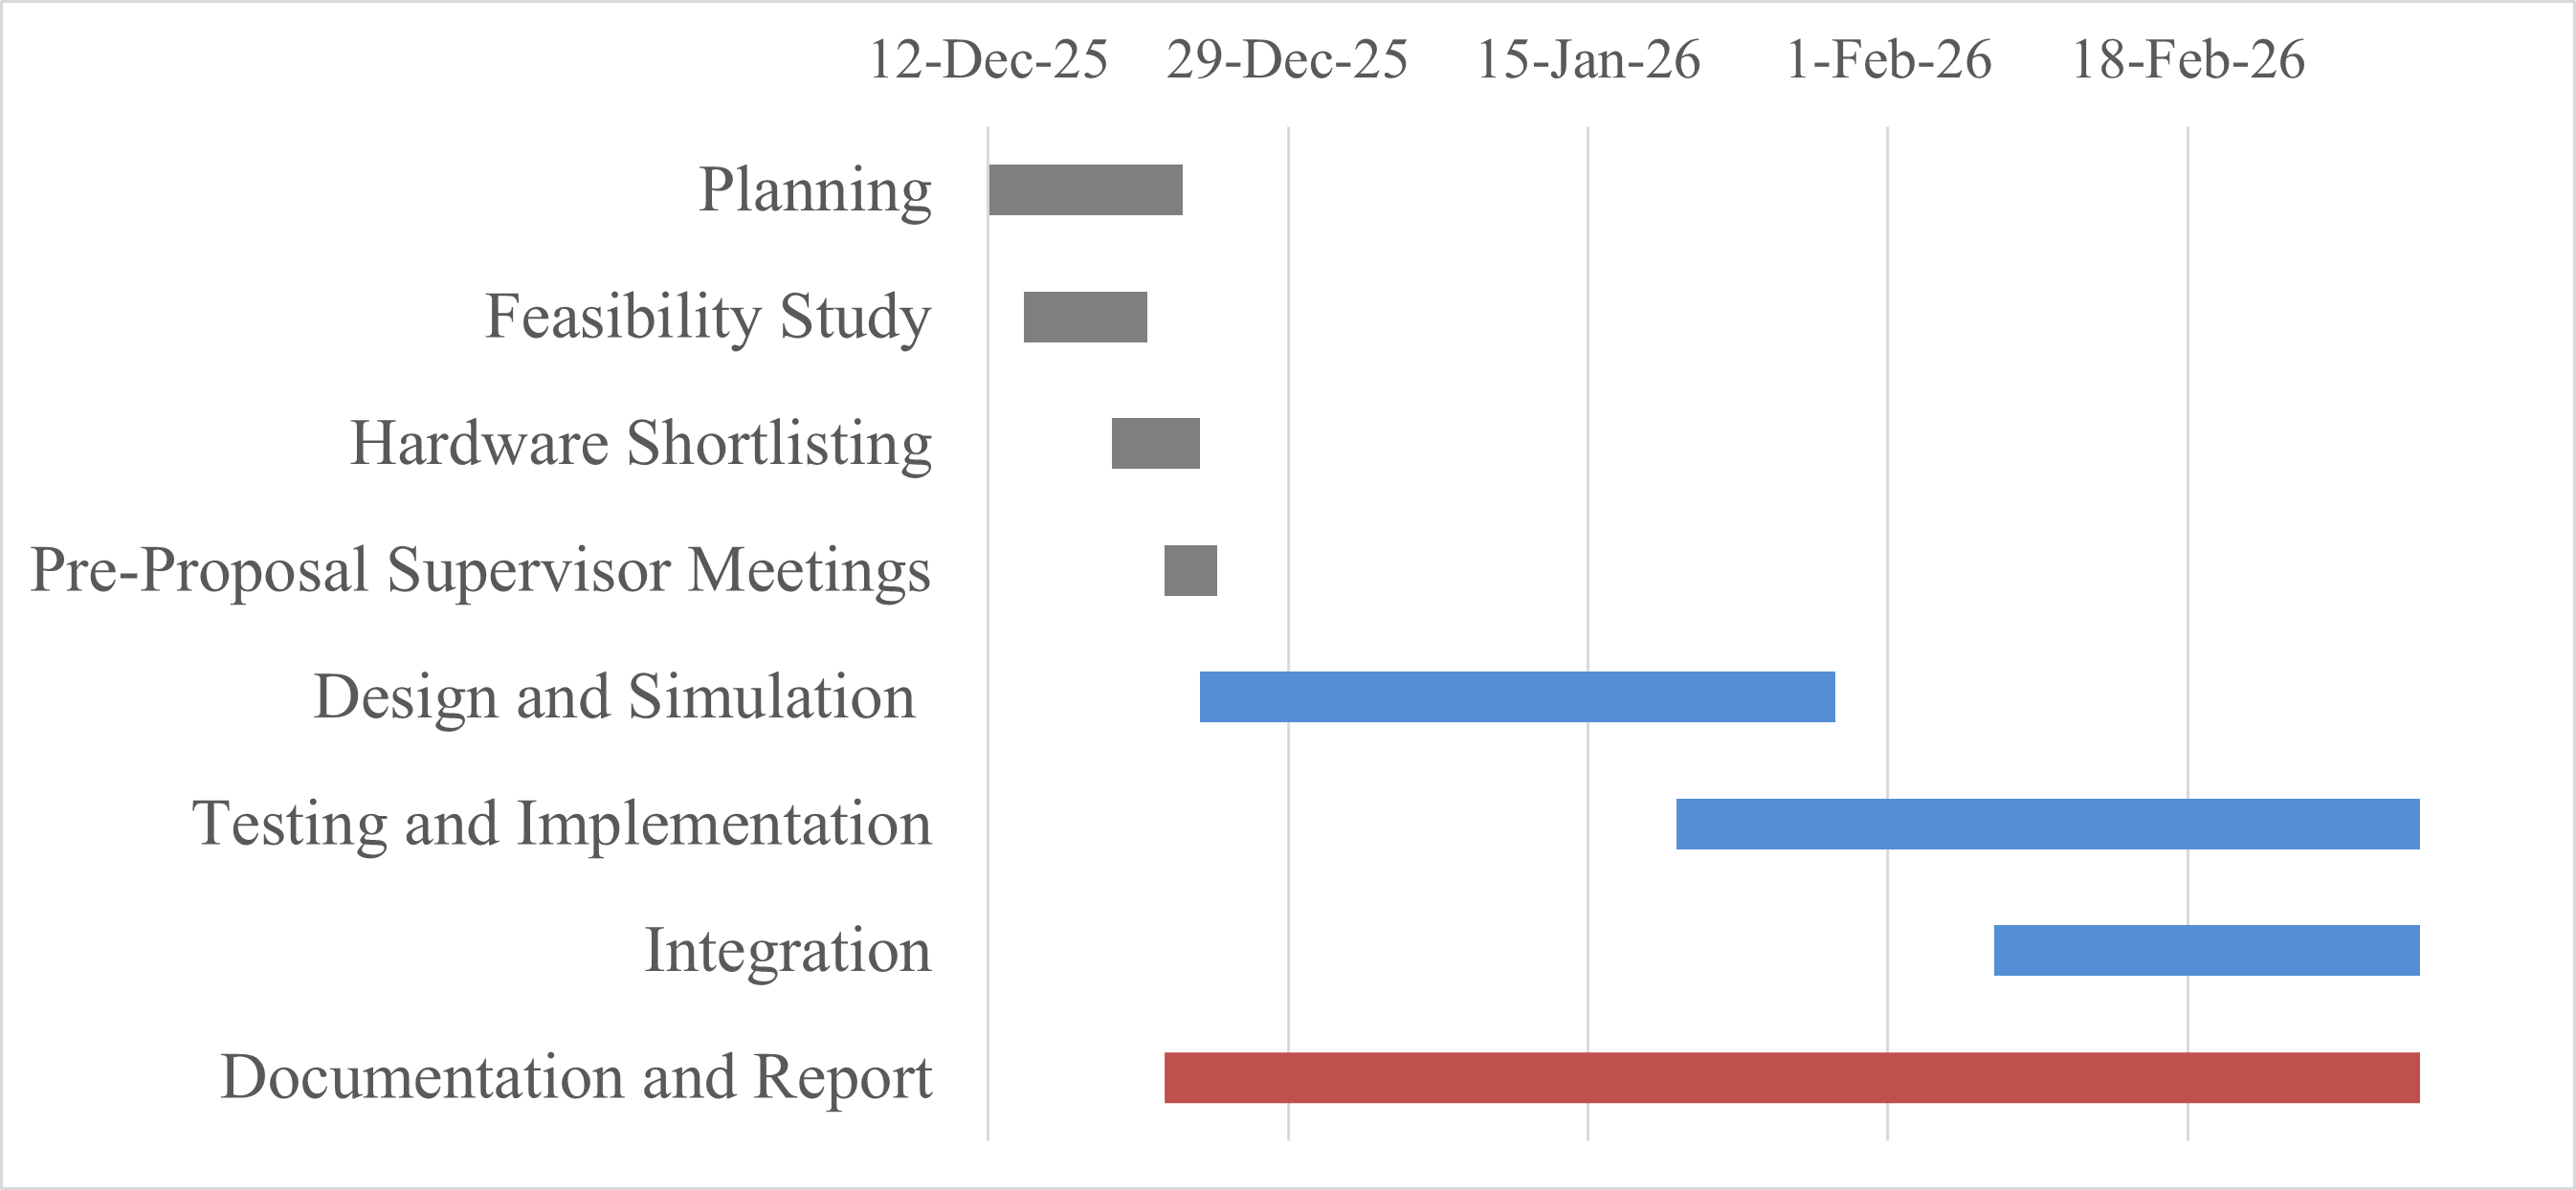
\includegraphics[width=\textwidth]{src/images/figures/gantt_chart.png}
	\caption{Project Gantt Chart}
	\label{gantt_chart}
\end{figure}
\newpage

\section{Budget Estimation}
\begin{table}[H]
	\centering
	\caption{Bill of Materials for EEG Acquisition Module}
	\begin{tabular}{|p{7.5cm}|c|c|c|}
		\hline
		\textbf{Component} & \textbf{Qty} & \textbf{Unit Cost} & \textbf{Total Cost} \\
		\hline
		Arduino Uno & 1 & 1000 & 1000 \\
		\hline
		AD620 Instrumentation Amplifier Module & 1 & 700 & 700 \\
		\hline
		LM741 Op-Amp IC & 3 & 40 & 120 \\
		\hline
		10~nF Capacitors & 5 & 10 & 50 \\
		\hline
		22~nF Capacitors & 5 & 10 & 50 \\
		\hline
		47~nF Capacitors & 5 & 10 & 50 \\
		\hline
		100~nF Capacitors & 5 & 10 & 50 \\
		\hline
		Resistor Box (Bundle of Resistors) & 1 & 175 & 175 \\
		\hline
		Gold Cup EEG Electrodes & 3 & 700 & 2100 \\
		\hline
		12~V Power Supply & 1 & 200 & 200 \\
		\hline
		Miscellaneous\textsuperscript{*} &  &  & 1000 \\
		\hline
		\multicolumn{3}{|r|}{\textbf{Total}} & \textbf{5495} \\
		\hline
	\end{tabular}
	\label{bill_of_materials}
\end{table}

\newpage
\section{Circuit Diagram}
\begin{figure}[H]
	\centering
	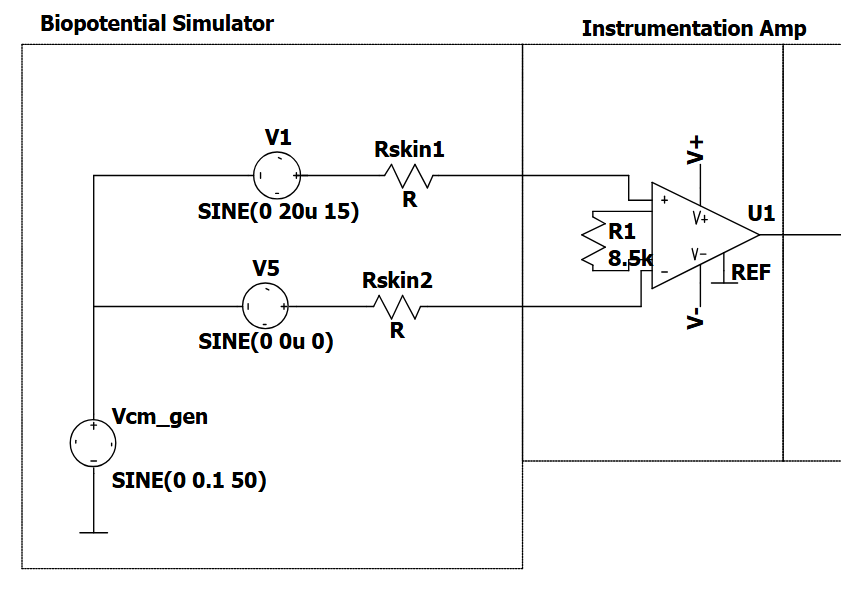
\includegraphics[width=\textwidth]{src/images/figures/ad620.png}
	\caption{AD620 (Instrumentation Amplifier)}
	\label{ina}
\end{figure}

\begin{figure}[H]
	\centering
	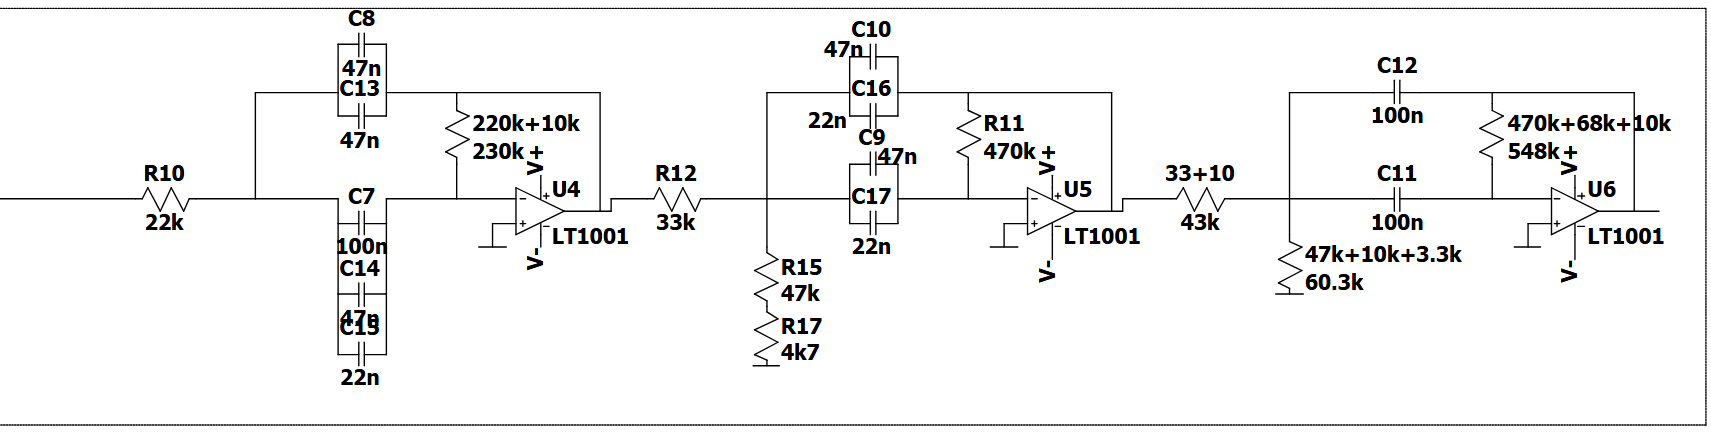
\includegraphics[width=20cm, height=7.5cm, angle = 90]{src/images/figures/filter_stage.png}
	\caption{$6^{\text{th}}$ order butterworth filter using lm741}
	\label{filter_circuit}
\end{figure}

\begin{figure}[H]
	\centering
	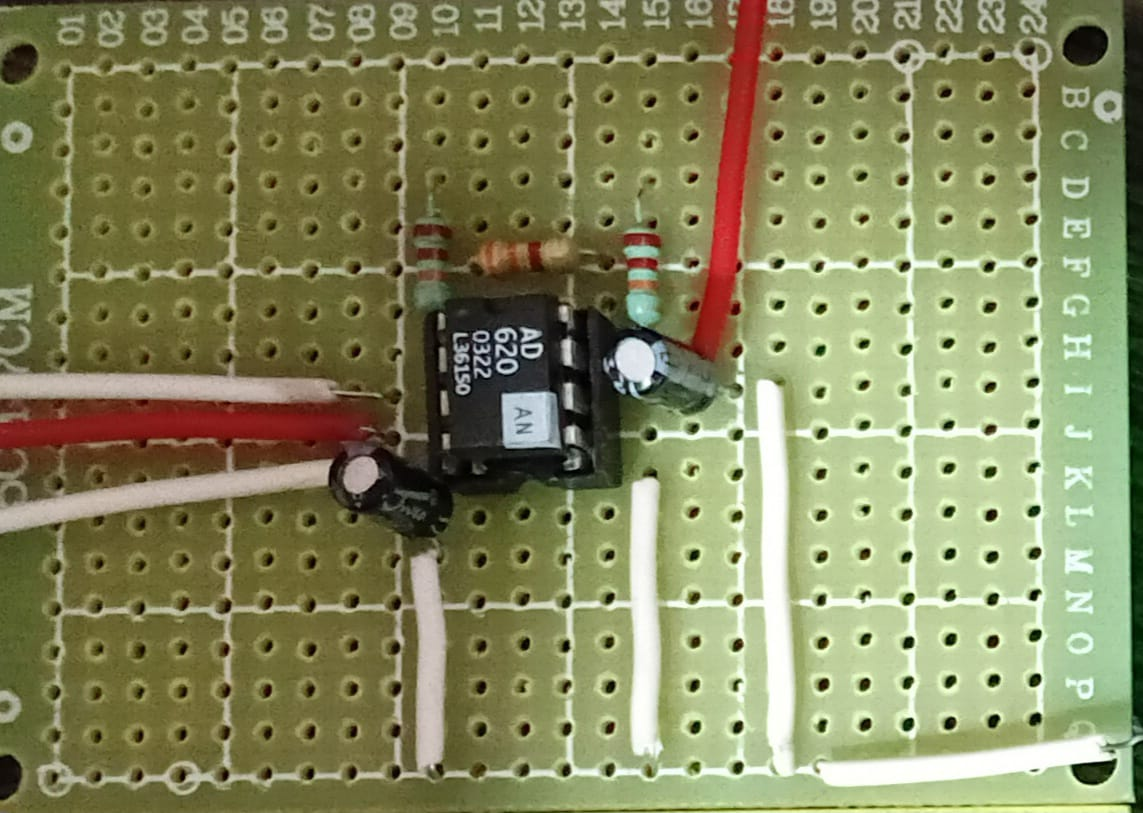
\includegraphics[width=10cm, height=7.5cm]{src/images/figures/ad620_h.jpg}
	\caption{AD620 Instrumentation Amplifier Circuit}
	\label{ad620_h}
\end{figure}

\begin{figure}[H]
	\centering
	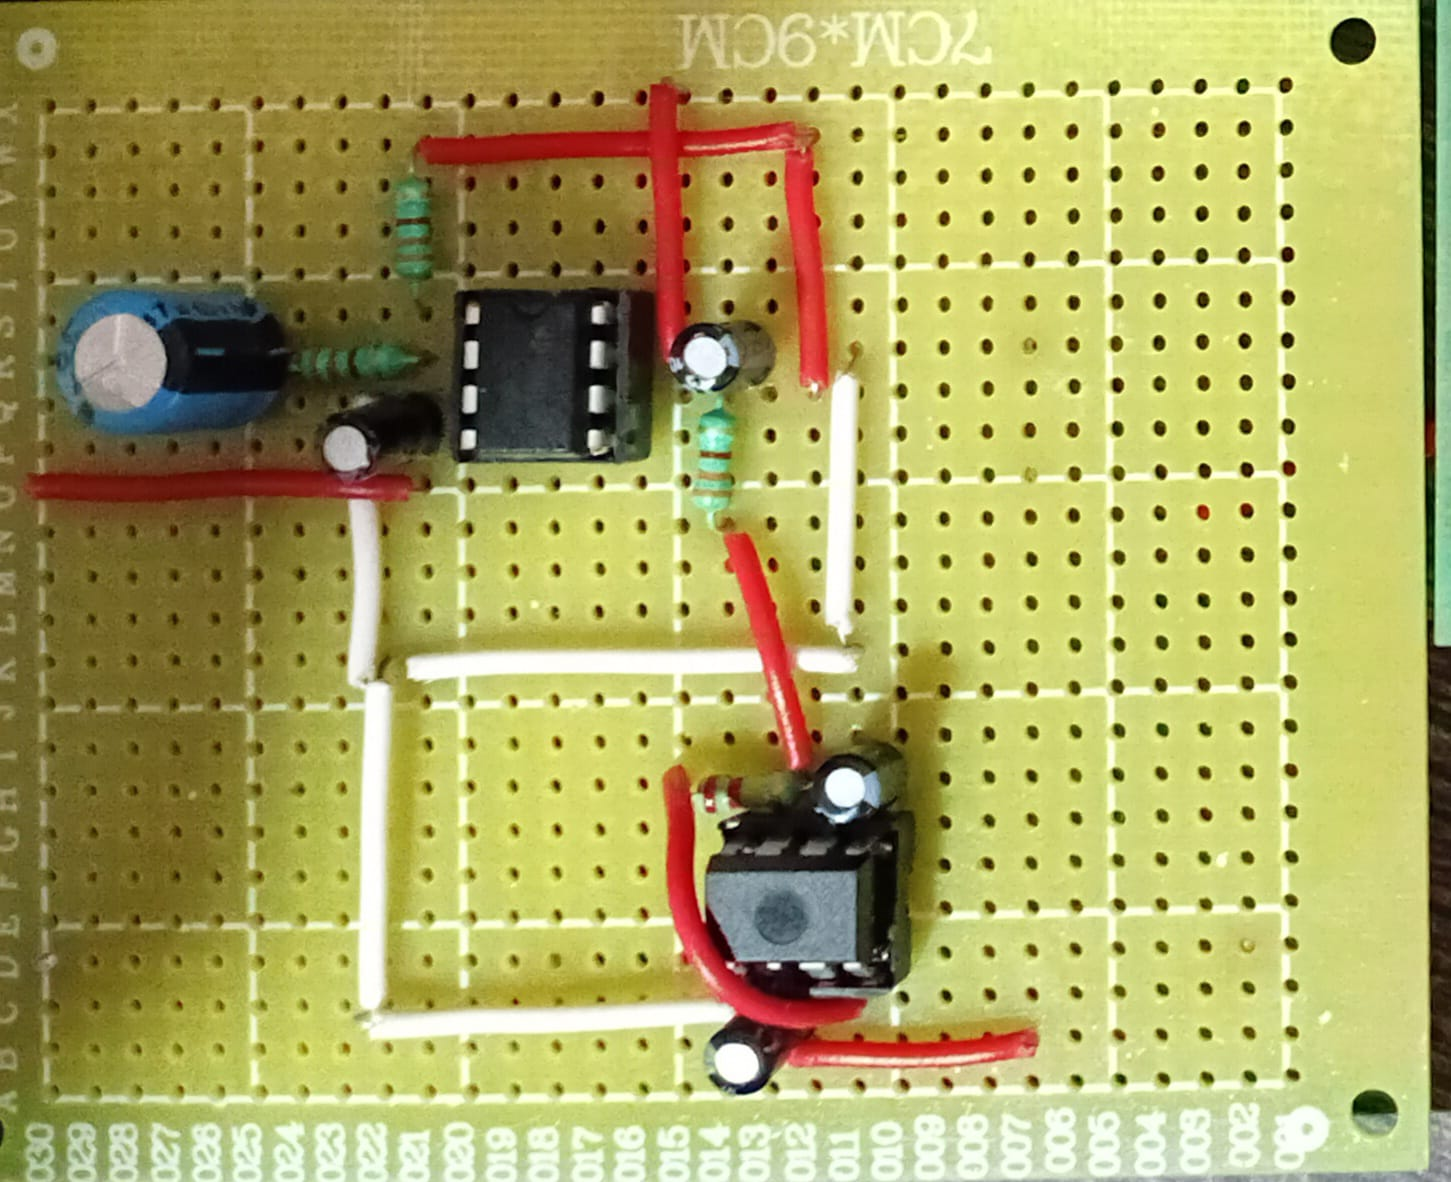
\includegraphics[width=10cm, height=7.5cm]{src/images/figures/high_pass_h.jpg}
	\caption{High Pass Filter Circuit}
	\label{high_pass_h}
\end{figure}

\begin{figure}[H]
	\centering
	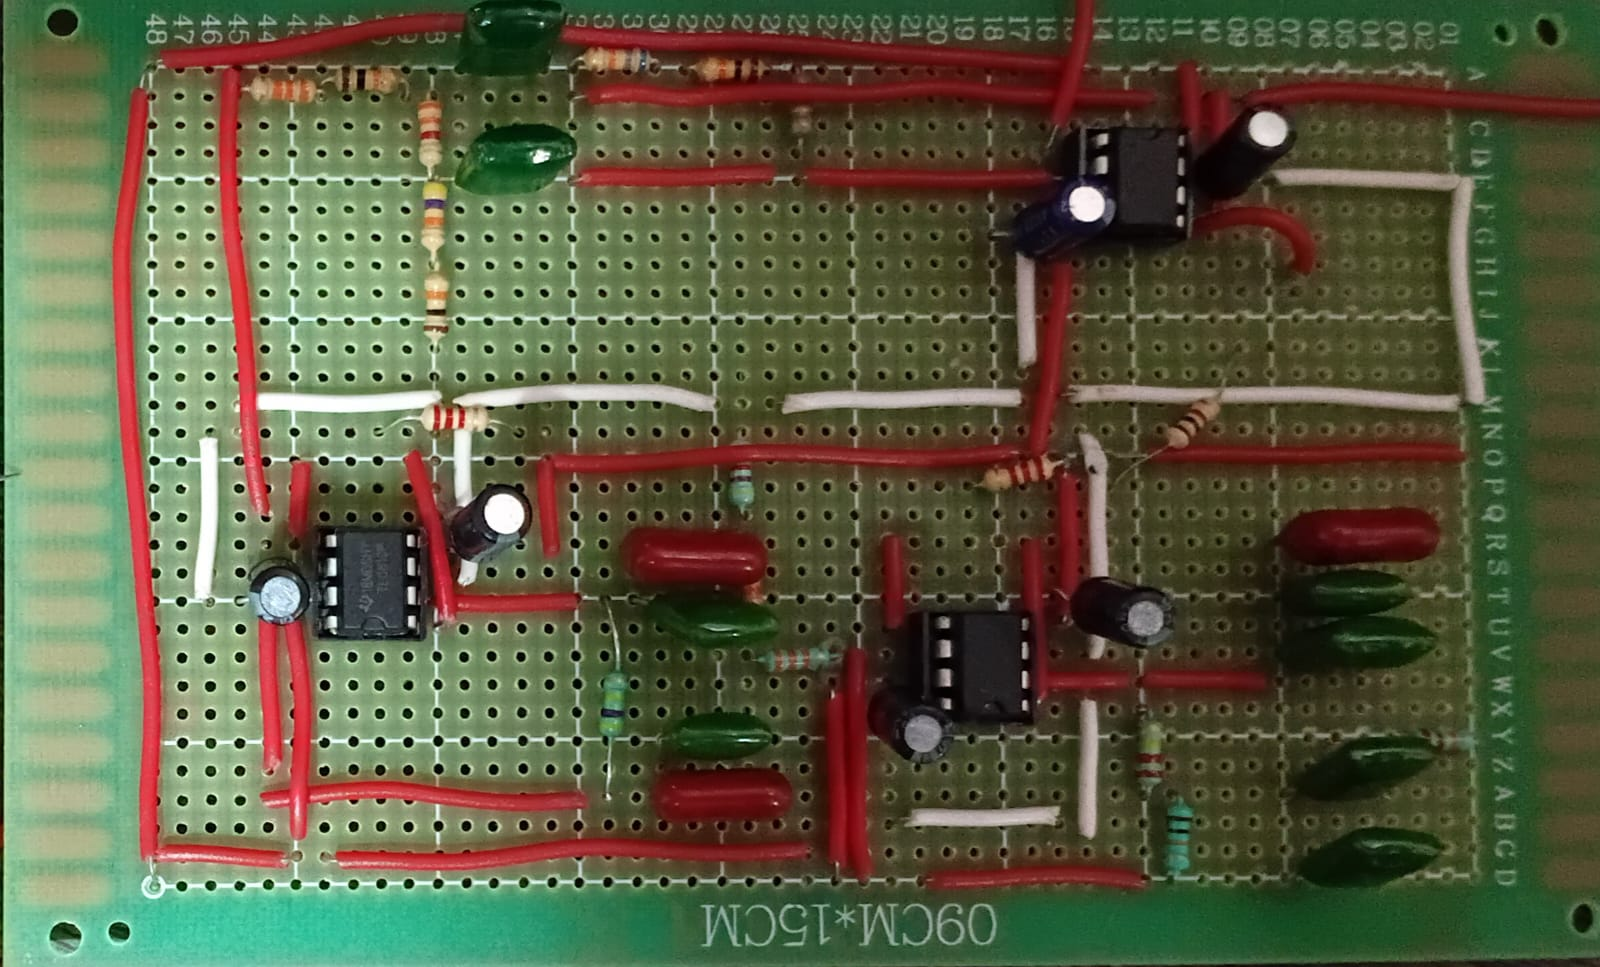
\includegraphics[width=10cm, height=7.5cm]{src/images/figures/3stage_h.jpg}
	\caption{Three Stage $6^{\text{th}}$ Order Band Pass Circuit}
	\label{3stage_h}
\end{figure}

\begin{figure}[H]
	\centering
	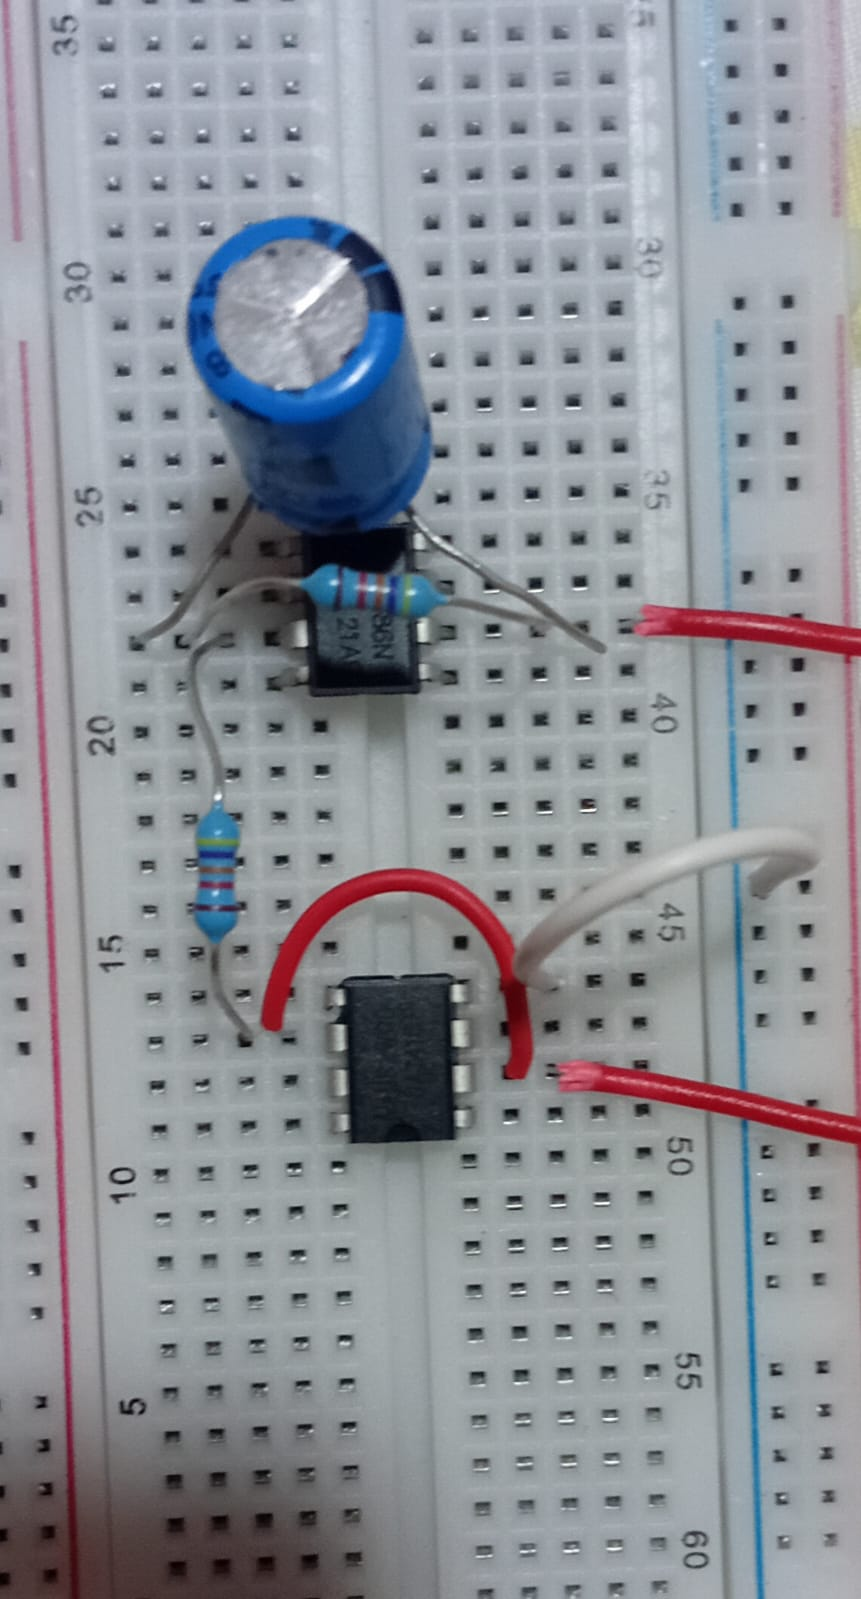
\includegraphics[width=10cm, height=7.5cm]{src/images/figures/drl_h.jpg}
	\caption{DRL Circuit}
	\label{drl_h}
\end{figure}


\newpage
\section{Module Specifications}

\subsection{EEG Signal Acquisition Module}
\begin{table}[H]
	\centering
	\small
	\caption{EEG Signal Acquisition Module}
	\begin{tabular}{p{6.5cm}p{6.5cm}ccc}
		\toprule
		\textbf{Parameter}                  & \textbf{Specification}   							\\
		\midrule
		Signal Type                     	& Electroencephalogram (EEG)						\\
		Number of Electrodes                & 3 (Fp1, Fp2, Reference)     						\\
		Electrode Type						& Ag/AgCl Surface Electrodes 						\\
		Input Signal Amplitude				& \SI{10}{\micro\volt} - \SI{100}{\micro\volt} 		\\
		Frequency 							& 0.5Hz - 40Hz 										\\
		Mode of Acquisition 				& Non invasive				 						\\
		\bottomrule
	\end{tabular}
	\label{eeg_signal_acq_module}
\end{table}


\subsection{Instrumentation Amplifier Module (AD620)}
\begin{table}[H]
	\centering
	\small
	\caption{Instrumentation Amplifier Module (AD620)}
	\begin{tabular}{p{6.5cm}p{6.5cm}}
		\toprule
		\textbf{Parameter} & \textbf{Specification} \\
		\midrule
		IC Used & AD620 \\
		Input Impedance & $\geq$ \SI{10}{\giga\ohm} \\
		CMRR & > 100 dB \\
		Gain Equation & \( G = 1 + \frac{49.4~\text{k}\Omega}{R_g} \) \\
		Supply Voltage & ±9 V \\
		Application & Low-level biopotential amplification \\
		\bottomrule
	\end{tabular}
\end{table}

\subsection{Signal Conditioning Module (Filters)}
\begin{table}[H]
	\centering
	\small
	\caption{Signal Conditioning Module (Filters)}
	\begin{tabular}{p{6.5cm}p{6.5cm}}
		\toprule
		\textbf{Filter Type} & \textbf{Specification} \\
		\midrule
		High-Pass Filter & Cut-off frequency = \SI{10}{\hertz} \\
		Low-Pass Filter & Cut-off frequency = \SI{40}{\hertz} \\
		Filter Order & Second order \\
		Purpose & Noise and artifact removal \\
		\bottomrule
	\end{tabular}
\end{table}

\subsection{Data Acquisition and Processing Module Specifications}
\begin{table}[H]
	\centering
	\small
	\caption{Data Acquisition and Processing Module Specifications}
	\begin{tabular}{p{6.5cm}p{6.5cm}}
		\toprule
		\textbf{Parameter} & \textbf{Specification} \\
		\midrule
		Microcontroller & Arduino Uno \\
		ADC Resolution & 10-bit \\
		Sampling Frequency & \SI{256}{\hertz} - \SI{1024}{\hertz} \\
		Input Voltage Range & 0 – 5 V \\
		Communication & USB Serial \\
		\bottomrule
	\end{tabular}
\end{table}

\subsection{EEG Signal Processing Module Specifications}
\begin{table}[H]
	\centering
	\caption{EEG Signal Processing Module Specifications}
	\begin{tabular}{p{5.5cm}p{8cm}}
		\toprule
		\textbf{Parameter} & \textbf{Specification} \\
		\midrule
		Programming Language & MATLAB \\
		Signal Processing & FFT based frequency analysis \\
		EEG Bands Analyzed & Beta Waves (10-30 Hz) \\
		Blink Detection & Amplitude threshold based \\
		Output & Text selection control \\
		\bottomrule
	\end{tabular}
	\label{tab:eeg_signal_processing}
\end{table}

\newpage

\section{Keyboard Interface}
\begin{figure}[H]
	\centering
	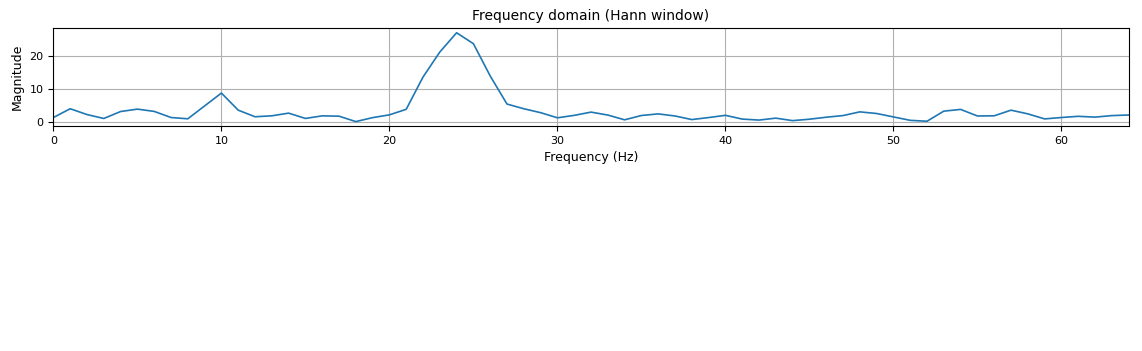
\includegraphics[width=\textwidth]{src/images/figures/keyboard_1.png}
	\label{keyboard_1}
\end{figure}
\begin{figure}[H]
	\centering
	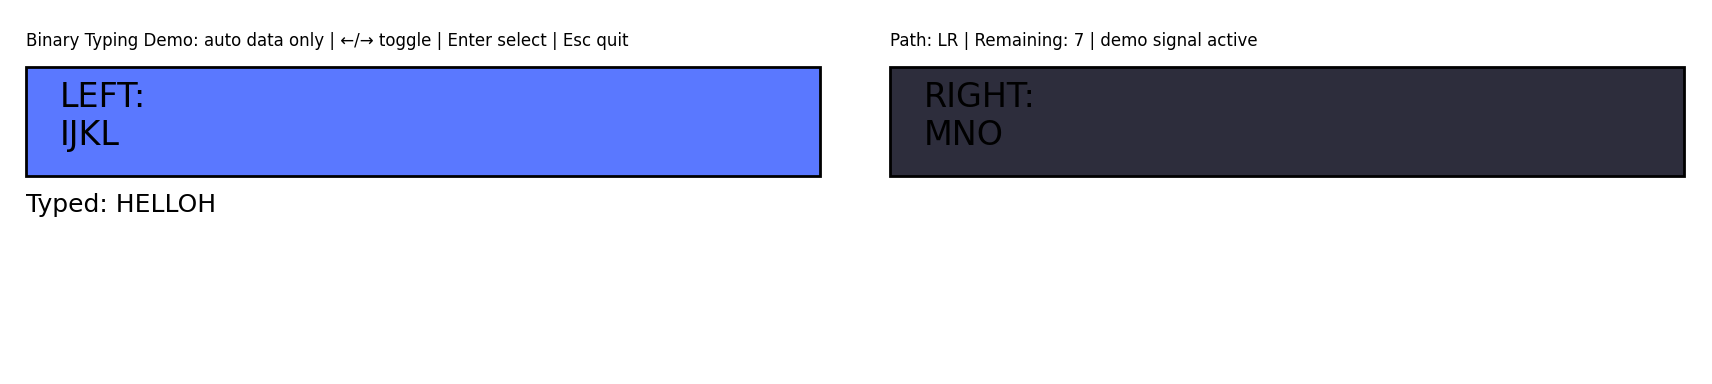
\includegraphics[width=\textwidth]{src/images/figures/keyboard_2.png}
	\caption{Keyboard Interface}
	\label{keyboard_2}
\end{figure}

\newpage
\section{Code Snippets}
\subsection{Keyboard Interface Code Snippet:}


\lstset{
	basicstyle=\ttfamily\footnotesize,
	frame=none,
	numbers=none,
	breaklines=true,
	columns=fullflexible,
	showstringspaces=false,
	keepspaces=true,
	tabsize=4,	
	backgroundcolor=\color{white},
	xleftmargin=0pt,
	framexleftmargin=0pt,
	keywordstyle=\relax,
	commentstyle=\relax,
	stringstyle=\relax,
	literate=
	{←}{{$\leftarrow$}}1
	{→}{{$\rightarrow$}}1
	{…}{{\ldots}}1
}

\begin{lstlisting}[language=Python]
	SYMBOLS = "ABCDEFGHIJKLMNOPQRSTUVWXYZ _<"
	
	class BinaryTyper:
	def __init__(self, symbols: str):
	self.all_symbols = list(symbols)
	self.reset_group()
	self.highlight = 0
	self.typed = ""
	
	def reset_group(self):
	self.group = self.all_symbols[:]
	self.path = []
	
	def split(self):
	mid = (len(self.group) + 1) // 2
	left = self.group[:mid]
	right = self.group[mid:]
	return left, right
	
	def toggle(self):
	self.highlight = 1 - self.highlight
	
	def select(self):
	left, right = self.split()
	chosen = left if self.highlight == 0 else right
	
	self.group = chosen
	self.path.append("L" if self.highlight == 0 else "R")
	self.highlight = 0
	
	if len(self.group) == 1:
	sym = self.group[0]
	
	if sym == "_":
	self.typed += " "
	elif sym == "<":
	self.typed = self.typed[:-1]
	else:
	self.typed += sym
	
	self.reset_group()
	
	def backspace(self):
	self.typed = self.typed[:-1]
	
	def previews(self):
	left, right = self.split()
	return left, right, len(self.group), "".join(self.path)
\end{lstlisting}


\lstdefinestyle{ArduinoStyle}{
	backgroundcolor=\color{white},   % white background for printing
	basicstyle=\ttfamily\footnotesize,
	keywordstyle=\color{codeblue}\bfseries,
	commentstyle=\color{codegreen}\itshape,
	stringstyle=\color{red},
	numbers=left,
	numberstyle=\tiny\color{codegray},
	stepnumber=1,
	numbersep=5pt,
	showstringspaces=false,
	breaklines=true,
	frame=none,
	captionpos=b
}

\subsection{Interrupt Service Setup and Routine}

\begin{lstlisting}[style=ArduinoStyle, language=C, caption={Interrupt Service Setup and Routine in Arduino for Sampling}, label={isr}]
	void setupTimer1_1024Hz(){
		cli();
		TCCR1A = 0;
		TCCR1B = 0;
		OCR1A = 31249;       // 16MHz -> 512Hz
		TCCR1B = 0x09;       // prescaler=1
		TIMSK1 = 0x02;       // enable OCR1A interrupt
		sei();
	}
	
	ISR(TIMER1_COMPA_vect){
		ADCSRA |= (1 << ADSC); 
		float sample = adc * ADC;
		sample-=5;
		
		circBuf[writeIndex] = sample;
		writeIndex = (writeIndex + 1) & (N - 1);
		
		samplesCollected++;
		if (samplesCollected >= N &&
		(((samplesCollected - N) & (HOP_SIZE - 1)) == 0)) {
			fftReady = true;
		}
	}
\end{lstlisting}

\newpage
\subsection{Code Snippet of FFT on Arduino}
\begin{lstlisting}[style=ArduinoStyle, language=C, caption={FFT Function}, label={fft}]
	void fft(float *real, float *imag){
		bitReversalPermutation(real, imag);
		
		for (uint8_t stage = 1; stage <= 7; stage++){
			uint8_t m = 1 << stage;
			uint8_t m2 = m >> 1;
			
			float theta = -2.0 * PI / m;
			float wm_real = fastCos(theta);
			float wm_imag = fastSin(theta);
			
			for (uint8_t k = 0; k < N; k += m){
				float w_real = 1.0;
				float w_imag = 0.0;
				
				for (uint8_t j = 0; j < m2; j++){
					uint8_t t = k + j + m2;
					uint8_t u = k + j;
					
					float tr = w_real * real[t] - w_imag * imag[t];
					float ti = w_real * imag[t] + w_imag * real[t];
					
					real[t] = real[u] - tr;
					imag[t] = imag[u] - ti;
					
					real[u] += tr;
					imag[u] += ti;
					
					// w = w * wm
					float temp = w_real;
					w_real = temp * wm_real - w_imag * wm_imag;
					w_imag = temp * wm_imag + w_imag * wm_real;
				}
			}
		}
	}
\end{lstlisting}

%\addcontentsline{toc}{chapter}{APPENDICES}
%\input{src/backmatter/back.tex}
%\input{src/backmatter/studentGuide.tex}


% =====================
% REFERENCES
% =====================

\clearpage
\renewcommand{\bibname}{REFERENCES}
\nocite{*} 
\bibliographystyle{IEEEtran}
\bibliography{references}

\end{document}
